\chapter{Experimental Results from Corroded Rebar Specimens}
The results from the experimental program are summarized in this chapter and the implications for structural design are evaluated.

\section{Measurement of corrosion level}

\subsection{Mass loss method}

The corrosion level of each specimen was measured after the time to corrode them had passed. The procedure consisted in removing the corrosion products from the surface of the specimens. The bars were then weighted and the mass loss was measured. Finally the corrosion level is defined as the mass loss divided by the initial mas as shown in \ref{eq:mass_loss_CL}.

\begin{equation}
    CL=\frac{m_{initial}-m_{final}}{m_{initial}}
    \label{eq:mass_loss_CL}
\end{equation}

\ref{tab:CL_mass_loss} shows the resulting corrosion level using the mass loss methodology. The resulting corrosion was significantly close to the target corrosion levels, and proved that the test setup successfully achieved the intended corrosion levels. The bars corresponding to CL=25\% did not achieved the intended corrosion level and achieved a corrosion level of 20\%. The reason for this discrepancy is due to the corrosion products of the accelerated corrosion process being on top of the surface of the rebars and therefore not permitting the corrosion process to continue. In addition one specimen for CL=15\% did not achieve the intended corrosion level, mainly due to a faulty welding of the stainless steel wire to the rebar. These extra bars were re-purposed to tension tests and BBT tension tests of turned down rebars.

\begin{table}[]
\caption{Corroded Level measured from mass loss in gauge length}
\label{tab:CL_mass_loss}
\begin{center}
\begin{tabular}{lcccc}
Specimen ID & Initial mass (g) & Final mass (g) & Mass loss (g) & CL (\%) \\ \hline
CL5-T-1\_3    & 1260.8           & 1197.5         & 63.3          & 5.0\%   \\
CL5-BBT-1\_3  & 1249.6           & 1199.8         & 49.9          & 4.0\%   \\
CL5-BBT-4-6   & 1255.3           & 1192.9         & 62.4          & 4.9\%   \\
CL10-T-1\_3   & 1244.0           & 1122.6         & 121.3         & 9.8\%   \\
CL10-BBT-1\_3 & 1248.7           & 1131.7         & 117.0         & 9.4\%   \\
CL10-BBT-4-6  & 1258.7           & 1143.1         & 115.7         & 9.2\%   \\
CL15-BBT-1\_3 & 1217.9           & 1052.3         & 165.6         & 13.6\%  \\
CL15-BBT-4-6  & 1265.5           & 1095.4         & 170.1         & 13.4\%  \\
CL20-T-1\_3   & 1251.2           & 1022.9         & 228.4         & 18.3\%  \\
CL20-BBT-1\_3 & 1245.1           & 1018.3         & 226.8         & 18.2\%  \\
CL20-BBT-4\_6  & 1272.3           & 1013.8         & 258.5         & 20.3\% 
\end{tabular}
\end{center}
\end{table}

\subsection{3D Scans method}

The 3d scan arm was used to obtain 3D model of the corroded rebars to determine the effective diameter in the gauge length of the specimens. The effective diameter was used to determine the stress strain relationships and the bending strain in the rebars. Figure X.X shows a sample of the 3D scans for CL=15\% and CL=20\%, this figure shows that the 3d scans captured with a high level of precision the imperfections on the surface of the rebars. 

From the 3d model, the volume in the gauge length was obtained, and assuming a sylindrical volume the effecive diamter can be obtained as expressed in eq x.x. Where $L_{o}$ is the length of the scanned gauge length. With the effective diameter, the corrosion level can be estimated as shown in Eq. X.X. Where $d_{o}$ refers to the initial diameter, which in the case of the specimens of this study, it corresponds to $d_{o}=19mm (0.75 in)$

\begin{equation}
    d_{eff}=\frac{V}{\frac{1}{4}\pi L_{o}}
    \label{eq:eff_diameter}
\end{equation}

\begin{equation}
    CL=1-(\frac{d_{eff}}{d_{o}})^2
    \label{eq:CL_diameter}
\end{equation}

The data collected from the 3D scans is summarized in \ref{tab:CL_3D_scans}. The results shown below show that the CL measured using this approached matches well with the intended corrosion level.

\begin{table}[]
\caption{Corroded Level measured from 3D Scans in gauge length}
\label{tab:CL_3D_scans}
\begin{tabularx}{1.0\textwidth} { 
   >{\raggedright\arraybackslash}X 
   >{\centering\arraybackslash}X 
  >{\centering\arraybackslash}X >{\centering\arraybackslash}X >{\centering\arraybackslash}X >{\centering\arraybackslash}X}
Specimen ID    & Volume ($mm^{3}$) & Height \newline ($mm$) & Diameter ($mm$) & 3D Scans CL (\%) & Average CL (\%) \\ \hline
CL5-T-1    & 47702                          & 179         & 18.4          & 6.50\%                        & \multirow{3}{*}{6.00\%}  \\
CL5-T-2    & 47388                          & 176.5       & 18.5          & 5.80\%                        &                          \\
CL5-T-3    & 44696                          & 166.1       & 18.5          & 5.60\%                        &                          \\
CL5-BBT-1  & 48389                          & 178.2       & 18.6          & 4.70\%                        & \multirow{3}{*}{4.80\%}  \\
CL5-BBT-2  & 48903                          & 178.2       & 18.7          & 3.70\%                        &                          \\
CL5-BBT-3  & 47876                          & 178.6       & 18.5          & 5.90\%                        &                          \\
CL5-BBT-4  & 48618                          & 178         & 18.6          & 4.20\%                        & \multirow{3}{*}{4.70\%}  \\
CL5-BBT-5  & 47984                          & 178.3       & 18.5          & 5.60\%                        &                          \\
CL5-BBT-6  & 48750                          & 178.6       & 18.6          & 4.20\%                        &                          \\
CL10-T-1   & 45281                          & 178.8       & 18.0          & 11.10\%                       & \multirow{3}{*}{11.30\%} \\
CL10-T-2   & 44658                          & 178.1       & 17.9          & 12.00\%                       &                          \\
CL10-T-3   & 45359                          & 178.1       & 18.0          & 10.60\%                       &                          \\
CL10-BBT-1 & 45815                          & 178.5       & 18.1          & 9.90\%                        & \multirow{3}{*}{9.70\%}  \\
CL10-BBT-2 & 47595                          & 182         & 18.2          & 8.20\%                        &                          \\
CL10-BBT-3 & 45364                          & 178.8       & 18.0          & 11.00\%                       &                          \\
CL10-BBT-4 & 46486                          & 178.9       & 18.2          & 8.80\%                        & \multirow{3}{*}{10.00\%} \\
CL10-BBT-5 & 45676                          & 178.7       & 18.0          & 10.30\%                       &                          \\
CL10-BBT-6 & 45353                          & 178.2       & 18.0          & 10.70\%                       &                          \\
CL15-BBT-1 & 43119                          & 178.8       & 17.5          & 15.40\%                       & \multirow{3}{*}{15.30\%} \\
CL15-BBT-2 & 41474                          & 169.7       & 17.6          & 14.20\%                       &                          \\
CL15-BBT-3 & 35373                          & 148.1       & 17.4          & 16.20\%                       &                          \\
CL15-BBT-4 & 40485                          & 168.1       & 17.5          & 15.50\%                       & \multirow{3}{*}{15.00\%} \\
CL15-BBT-5 & 38297                          & 160.4       & 17.4          & 16.20\%                       &                          \\
CL15-BBT-6 & 41103                          & 166.4       & 17.7          & 13.30\%                       &                          \\
CL20-T-1   & 40786                          & 178.2       & 17.1          & 19.70\%                       & \multirow{3}{*}{20.30\%} \\
CL20-T-2   & 36577                          & 163.4       & 16.9          & 21.40\%                       &                          \\
CL20-T-3   & 40864                          & 178.6       & 17.1          & 19.70\%                       &                          \\
CL20-BBT-1 & 41038                          & 178.9       & 17.1          & 19.50\%                       & \multirow{3}{*}{19.50\%} \\
CL20-BBT-2 & 37452                          & 164.3       & 17.0          & 20.00\%                       &                          \\
CL20-BBT-3 & 41186                          & 178.5       & 17.1          & 19.00\%                       &                          \\
CL20-BBT-4 & 39645                          & 178.4       & 16.8          & 22.00\%                       & \multirow{3}{*}{21.80\%} \\
CL20-BBT-5 & 35364                          & 158.4       & 16.9          & 21.70\%                       &                          \\
CL20-BBT-6 & 39786                          & 178.1       & 16.9          & 21.60\%                       &                                                                             
\end{tabularx}
\end{table}

\subsection{Comparison of corrosion level measurements mass loss vs 3D scans}

Finally, the results from obtaining the corrosion level using the mass loss approach and the 3D scans are compared in Fig x.x the results from both approaches match very well, and the discrepancy from both can be due to more localized corrosion measured in the single specimens than those measured in the parent bar specimen as was the case for the mass loss methodology. These results provided us with the opportunity to use the measured effective diameter from the 3d scans into the tension tests and BBT tests described in the following sections.

\begin{figure}[htbp]
	\centering
    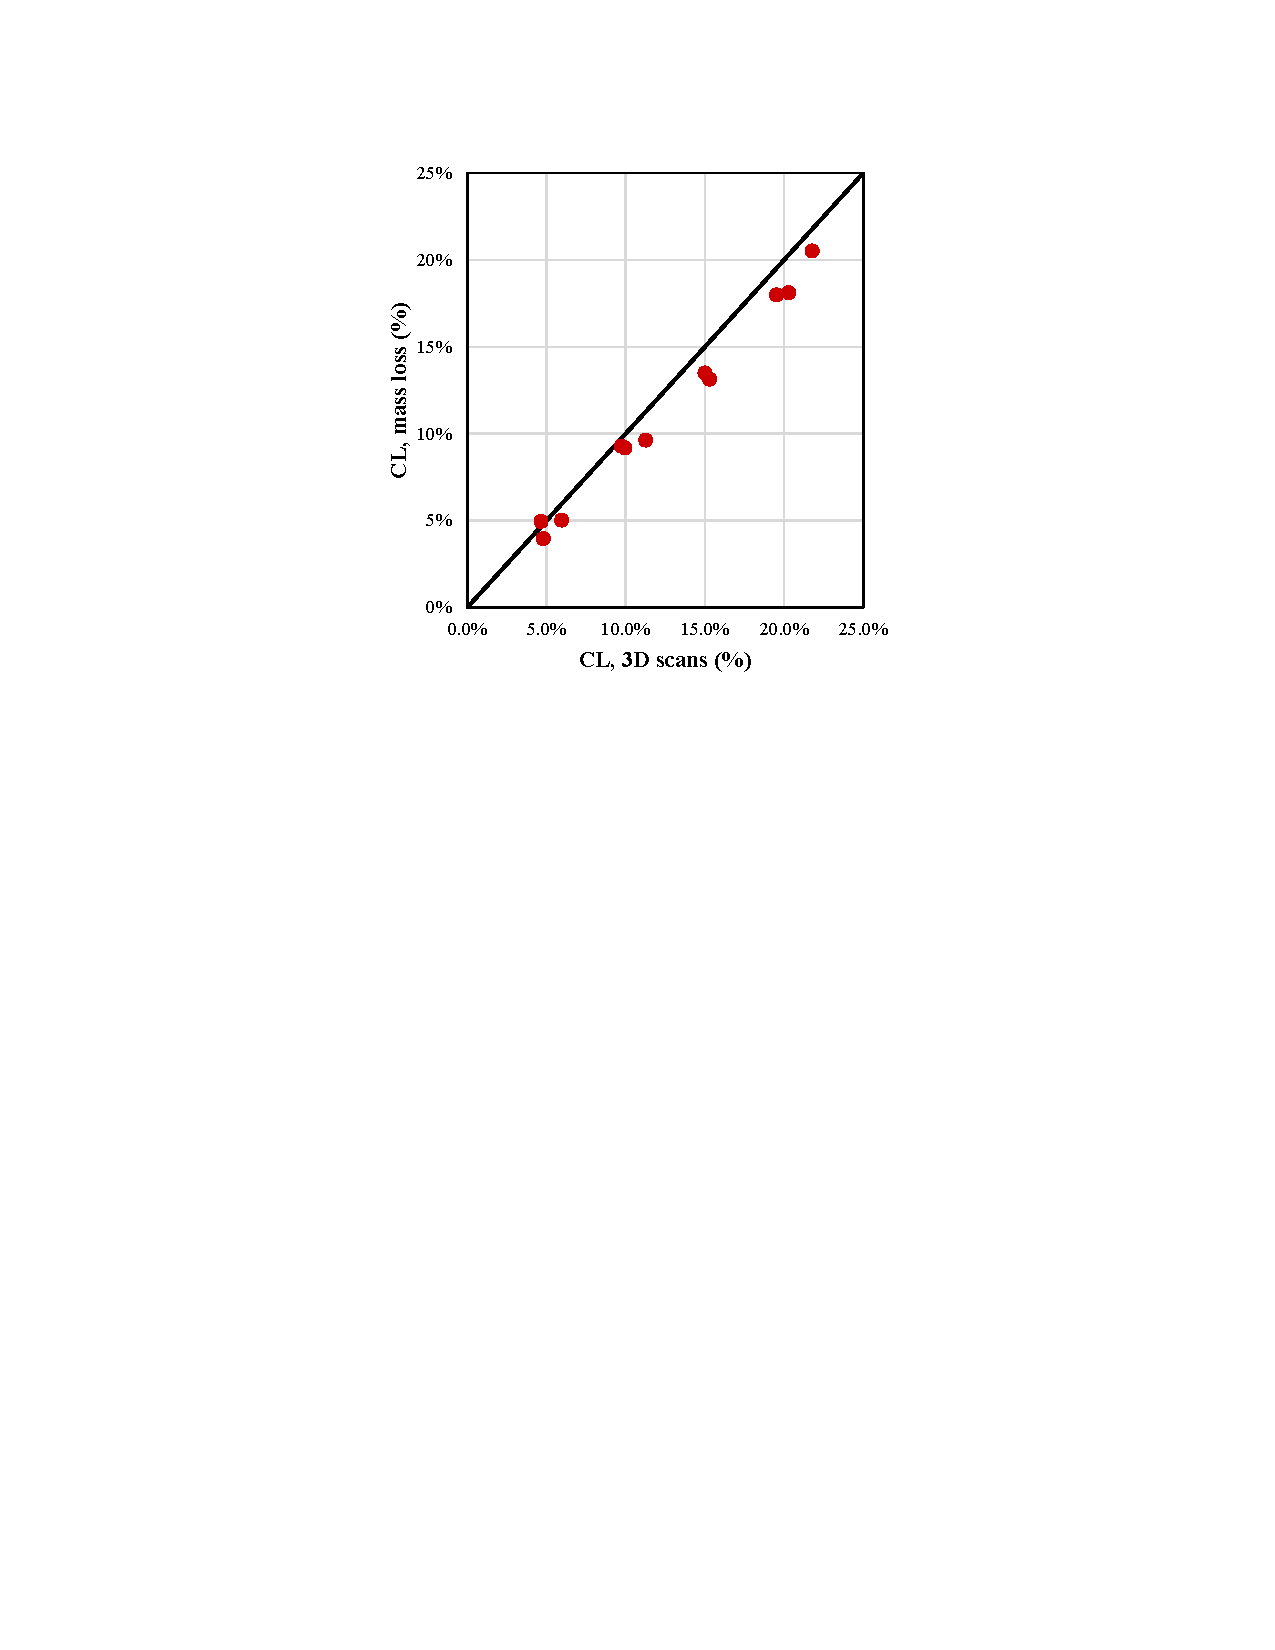
\includegraphics[width=0.7\textwidth]{VAC Thesis 2.0/Chapter-4/figs/3dscans_vs_massloss.pdf}
	\caption{Corrosion level (CL) measured using mass loss method vs 3D scans}
\label{fig:3dscans_vs_massloss}
\end{figure}

\section{Tensions Tests}

As described in Chapter 3, the bars were loaded in tension using the universal testing machine (UTM). The data collected corresponded to the Force using the UTM and the Optotrack system was used to calculate the strain.

During the tests it was observed that the failure usually occurred close to the grips. This is due to the sudden change in the cross section and the imperfections on the rebars. The strains used in this study correspond to the strain gauges located adjacent to the fracture. The fracture of these tests were brittle in nature, the appearance of necking was not significantly observable as shown in \fref{fig:TensionTest_NoNecking}.

\begin{figure}[htbp]
	\centering
	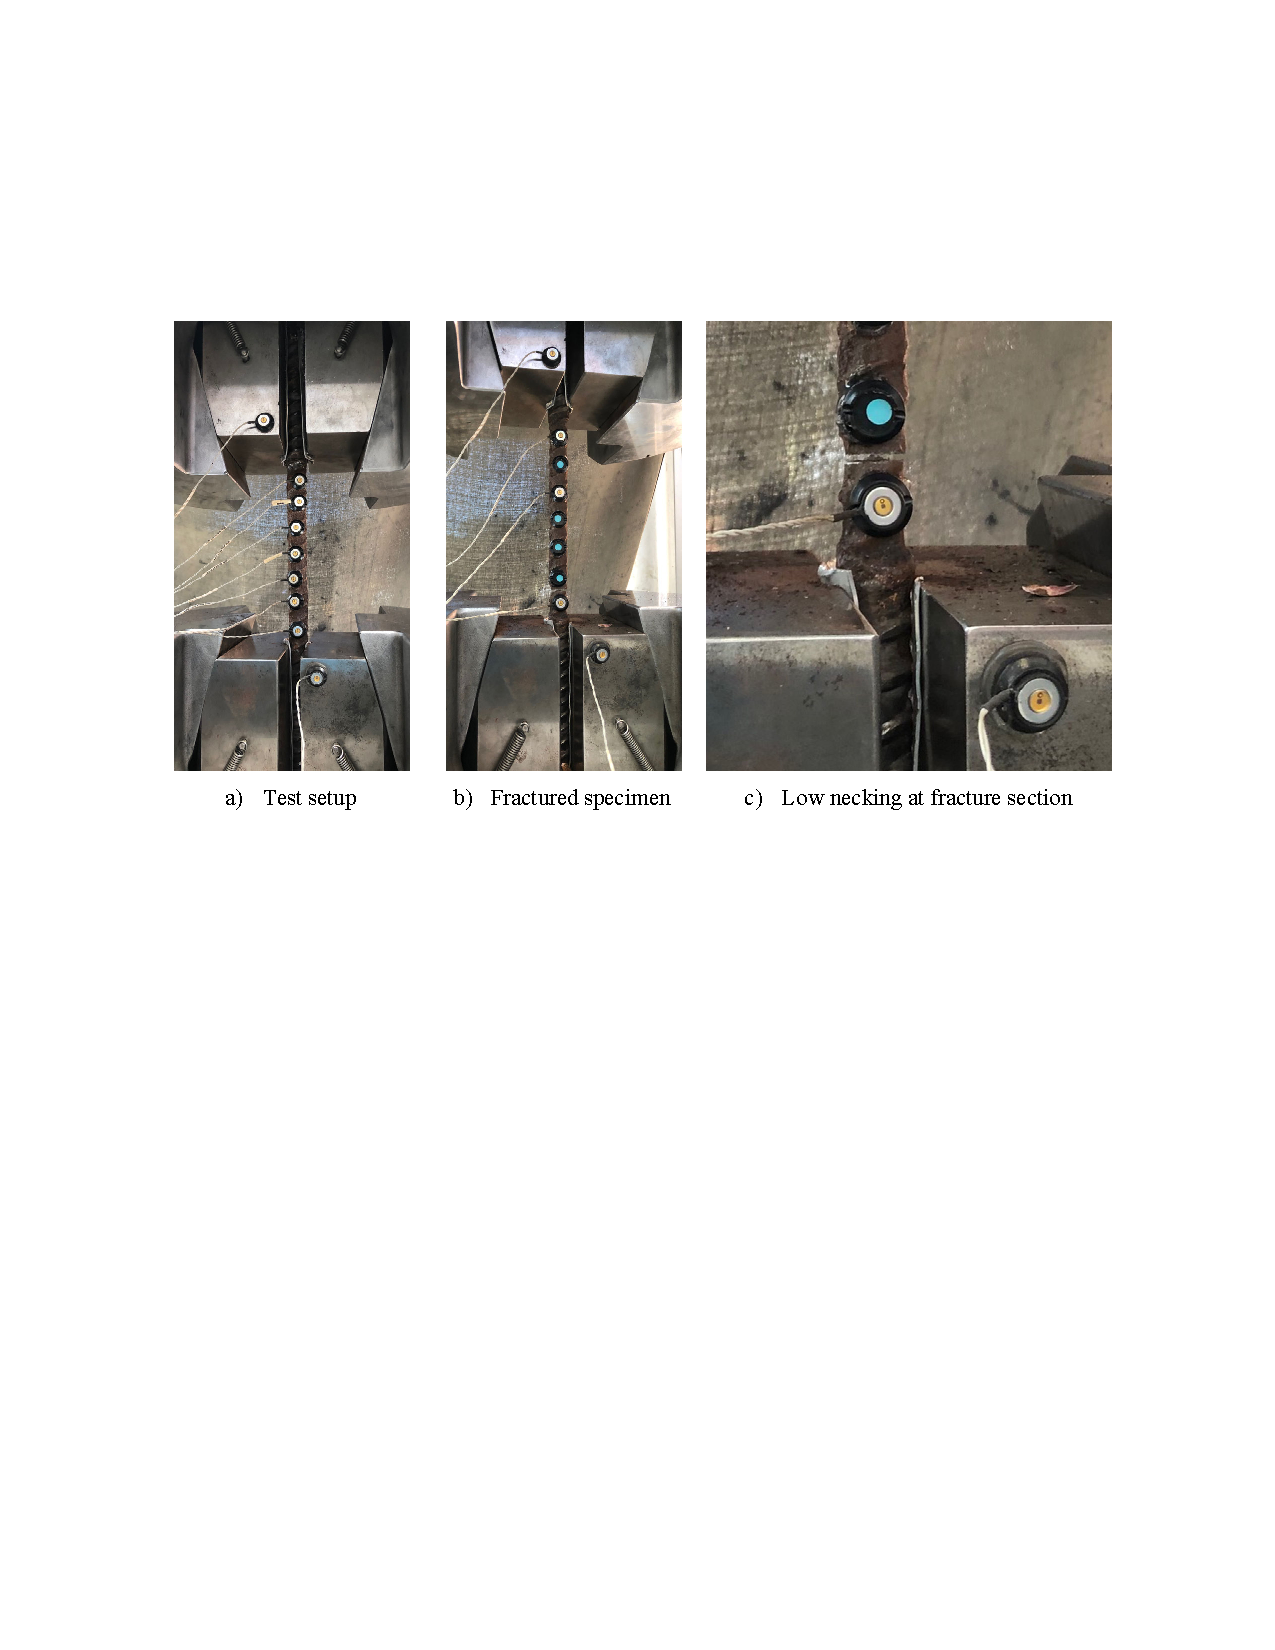
\includegraphics[width=0.7\textwidth]{VAC Thesis 2.0/Chapter-4/figs/TensionTest_images.pdf}
	\caption{Tension test setup and fracture observations}
	\label{fig:TensionTest_NoNecking}
\end{figure}

\fref{fig:TensionTestResults_StressStrain} show the stress-strain behavior for corrosion levels raging from 0 - 20\%. From this results, the yield strength, the uniform axial elongation, and the ultimate strength are obtained From this results it appears that the effective yield strength and the effective ultimate strength reduce as the corrosion level increases. In addition, the stress strain curves  results confirm that no necking significant necking was present, since were the after reaching the ultimate stress the bars suddenly drop  in strength. 

\begin{figure}[htbp]
	\centering
	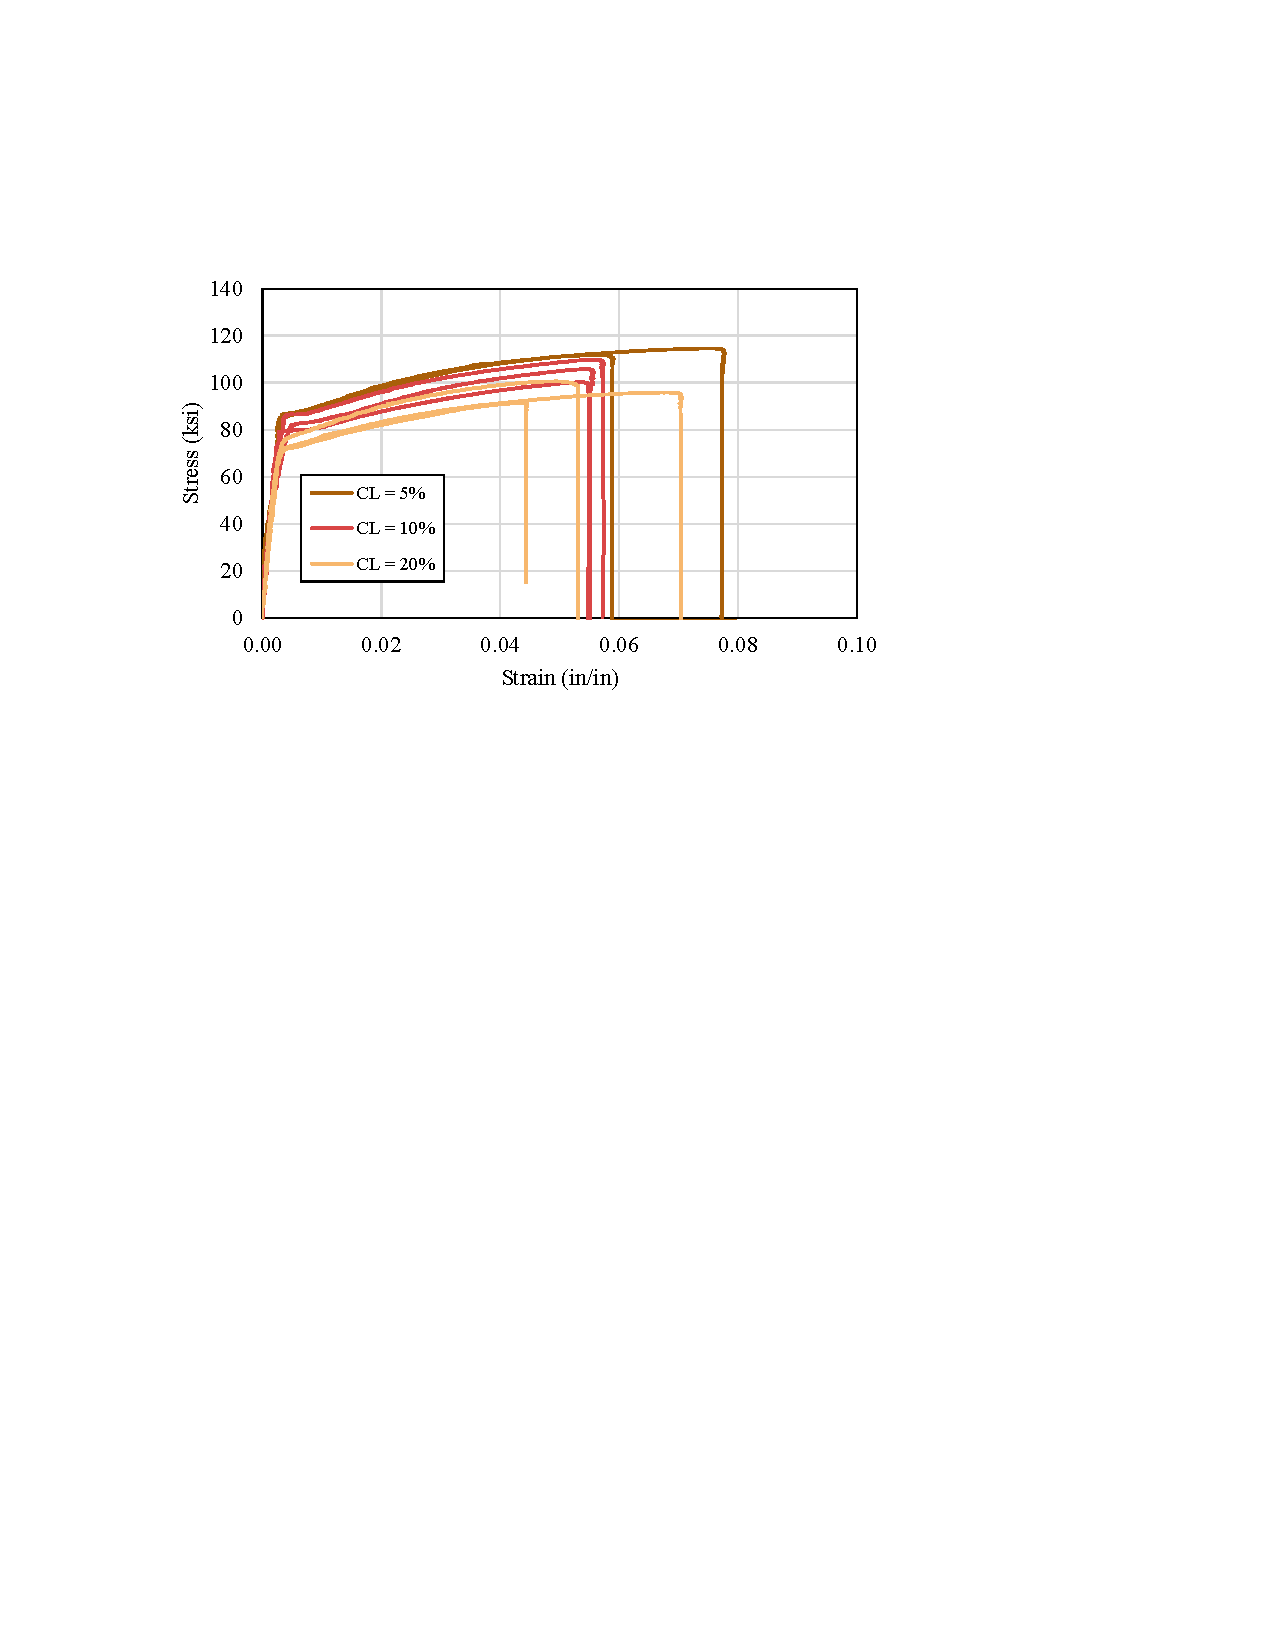
\includegraphics[width=0.7\textwidth]{VAC Thesis 2.0/Chapter-4/figs/TensionTest_results_1.pdf}
	\caption{Tension test results at different corrosion levels}
	\label{fig:TensionTestResults_StressStrain}
\end{figure}

\subsection{Yield strength as a function of corrosion}
\fref{fig:YieldStrength_vs_CL} shows the plot of the effective yield strength versus the corrosion level. The results show that there appears to be a linear relationship between them. This is congruent with other studies performed in other types of steel such as the study done by Du et al \cite{Du2005}. It has been studied that the apparent reduction in effective yield strength is due to points of concentrated reduction in the geometry of the rebars. Other studies \cite{Du2005}\cite{Barcley2018} and this study, show that if the imperfections due to the corrosion are removed, then the properties of the virgin metal remain unchanged. What is observed in tension tests conducted on corroded rebars is an effective property that considers the imperfections in the geometry of the rebar. 

The linear trend observed between the effective yield strength and the corrosion level can be expressed as:

\begin{equation}
    f_{y,CL} = f_{y,o}(1-0.0075CL)
    \label{eq.Calderon_Fy_vs_CL}
\end{equation}

\begin{figure}[htbp]
	\centering
	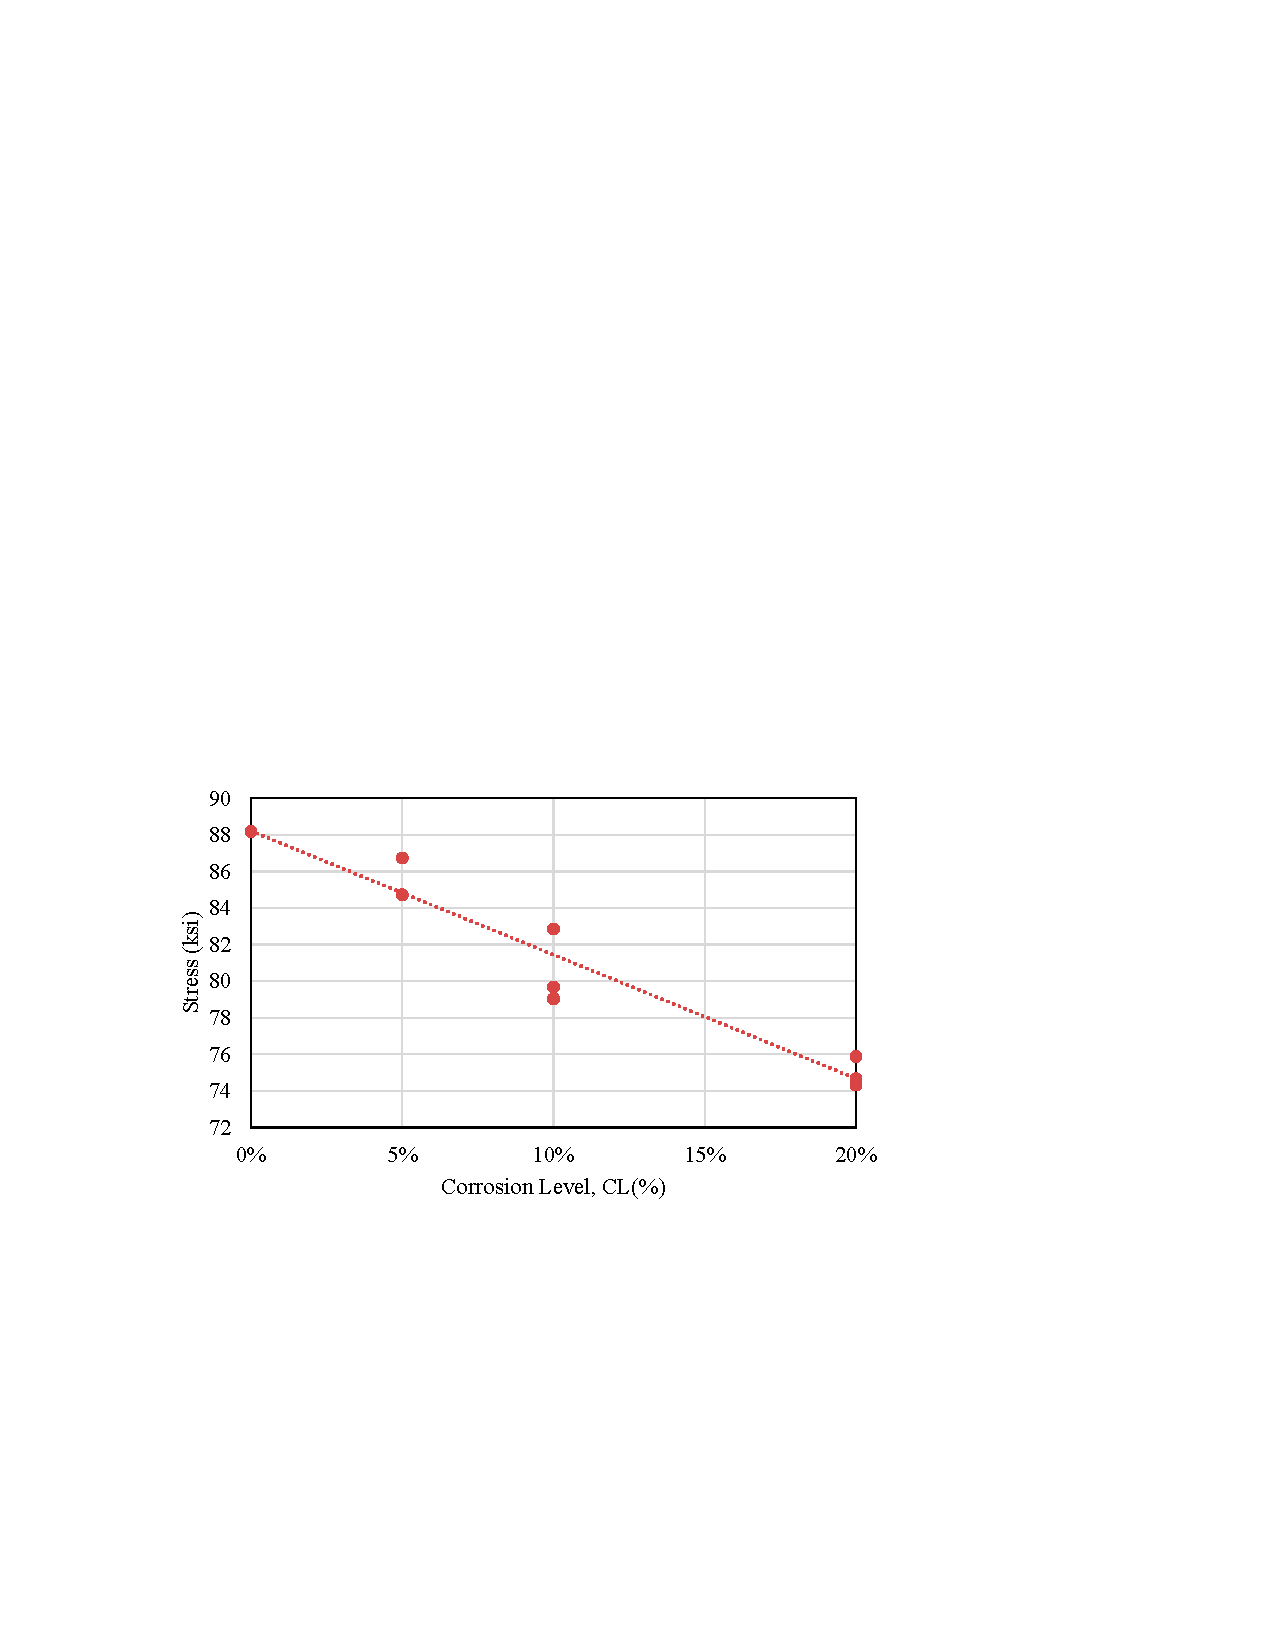
\includegraphics[width=0.7\textwidth]{VAC Thesis 2.0/Chapter-4/figs/TensionTest_results_2.pdf}
	\caption{Yield strength as a function of corrosion level}
	\label{fig:YieldStrength_vs_CL}
\end{figure}

The proposed equation is compared to the one proposed by Du et al \cite{Du2005}, replicated here as \ref{}. From \fref{fig:Calderon_vs_Du} we can observe that the existing model tends to over-predict the effective yield strength for Grade 80 steel. Therefore it is possible that there is correlation between corrosion level and the grade of the rebar, however the literature on corrosion for different grades of rebar is scarce. 

\begin{figure}[htbp]
	\centering
	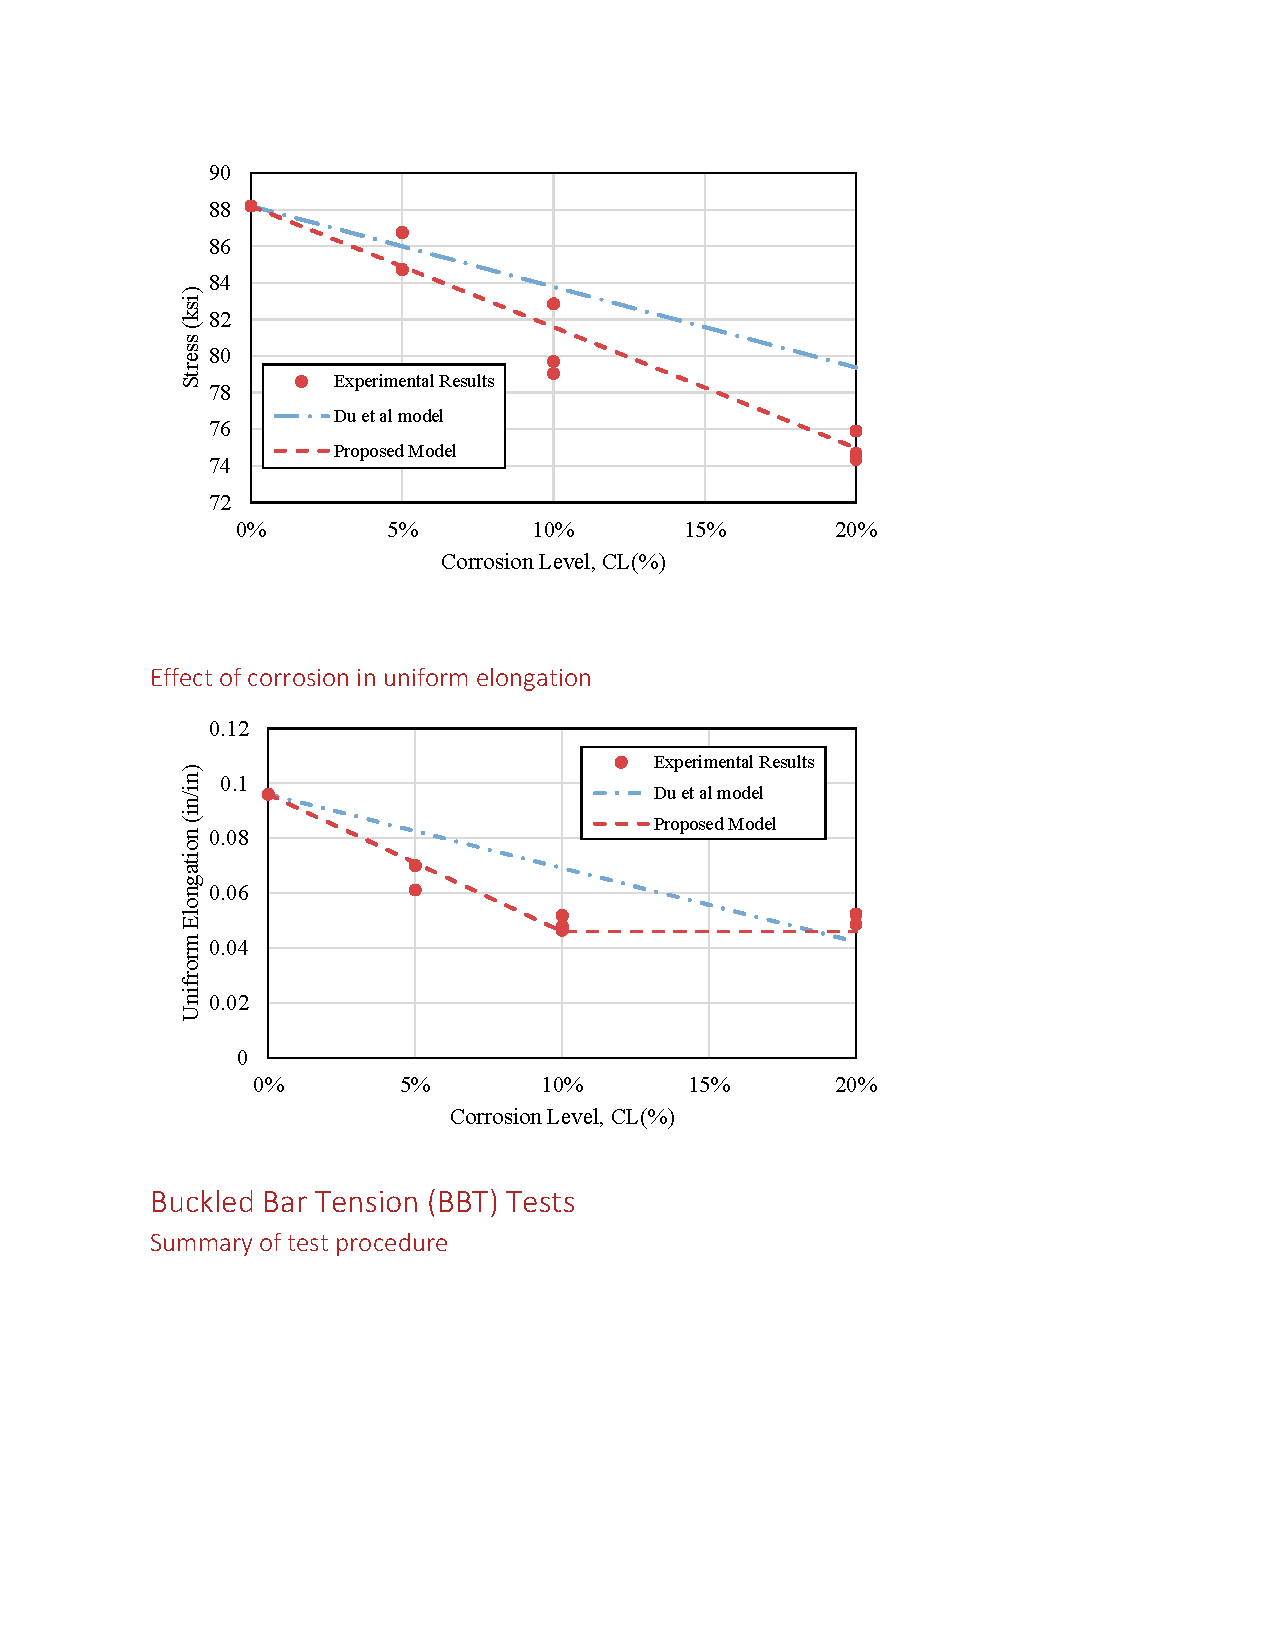
\includegraphics[width=0.7\textwidth]{VAC Thesis 2.0/Chapter-4/figs/TensionTest_results_3_proposedmodel.pdf}
	\caption{Yield strength as a function of corrosion level comparison of proposed model and Du et al model \cite{Du2005}}
	\label{fig:Calderon_vs_Du}
\end{figure}

\subsection{Effect of corrosion in uniform elongation}

Another interesting result was observed on the uniform axial elongation property of the corroded rebars. As the rebar corrodes and develops more imperfections on the geometry of the rebar, it appears that the uniform axial elongation decreases.\fref{fig:UAE_vs_CL} shows this trend more clearly. However, after 10\% corrosion the uniform axial elongation remains constant. This results may point towards why as structure corrode the level of perceived ductility is reduced and thus triggers an earlier failure than that observed on pristine structures.

We propose the following model to predict the uniform axial elongation of corroded grade 80 rebars:

For corrosion level between 0\% - 10\%
\begin{equation}
    \varepsilon_{CL} = \varepsilon_{o}-0.05CL
    \label{eq.Calderon_UAE_vs_CL}
\end{equation}

For corrosion level larger than 10\%

\begin{equation}
    \varepsilon_{CL} = 0.045
    \label{eq.Calderon_UAE_vs_CL20}
\end{equation}

While equations \ref{eq.Calderon_Fy_vs_CL} - \ref{eq.Calderon_UAE_vs_CL20} are preliminary they provide an insight at the variations that different grades of rebar can have on the effective properties of corroded rebars.

\begin{figure}[htbp]
	\centering
	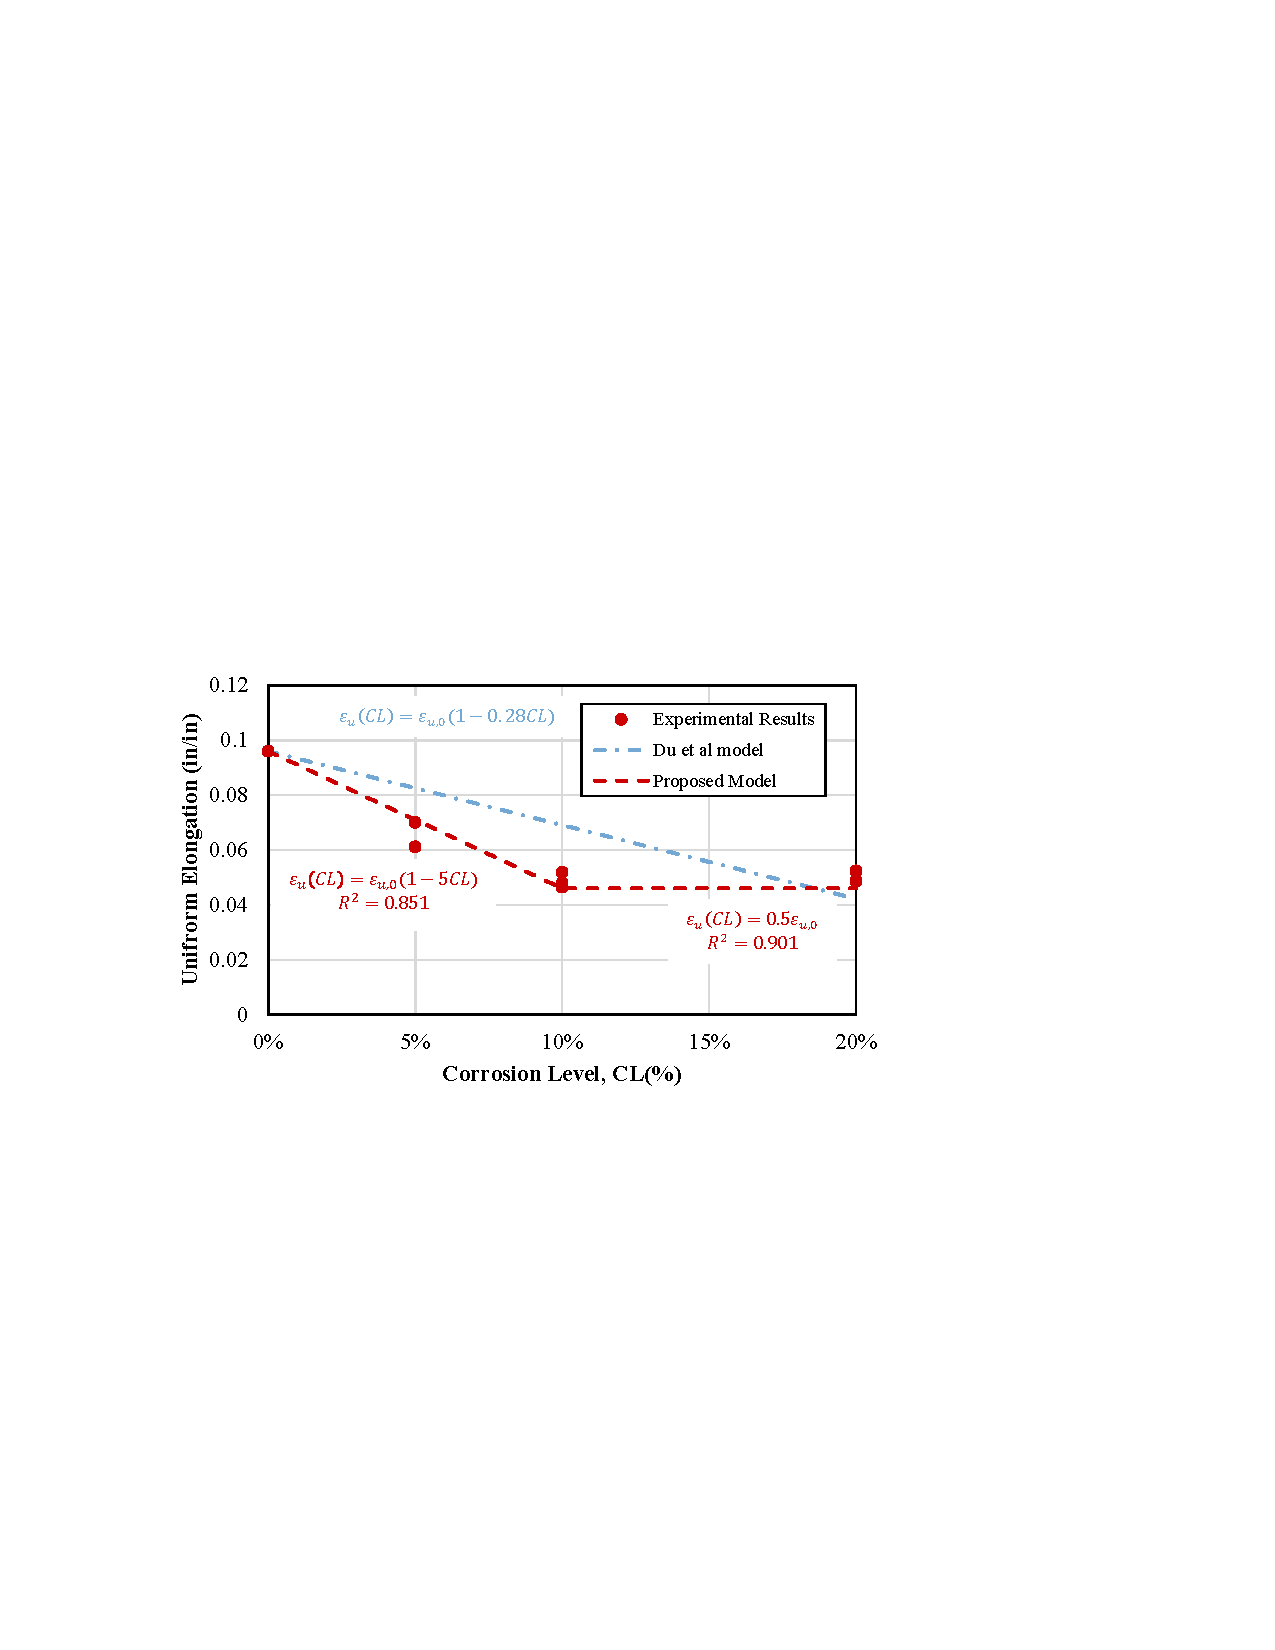
\includegraphics[width=0.7\textwidth]{VAC Thesis 2.0/Chapter-4/figs/TensionTest_results_4_proposedmodel.pdf}
	\caption{Uniform elongation as a function of the corrosion level comparison of proposed model and Du et al model \cite{Du2005}}
	\label{fig:UAE_vs_CL}
\end{figure}

\section{Buckled Bar Tension (BBT) Tests}
\subsection{Summary of BBT procedure}

The process of  performing the buckled bar test consists of: 1) Loading the bar with the LED markers in the UTM machine. 2) Compress the bars to a prescribed level of bending strain. 3) Load the rebar in tension and  4) Record the type of fracture: Ductile or Brittle. This process is presented in \fref{fig:BBT_Test_Summary}.

\begin{figure}[htbp]
	\centering
	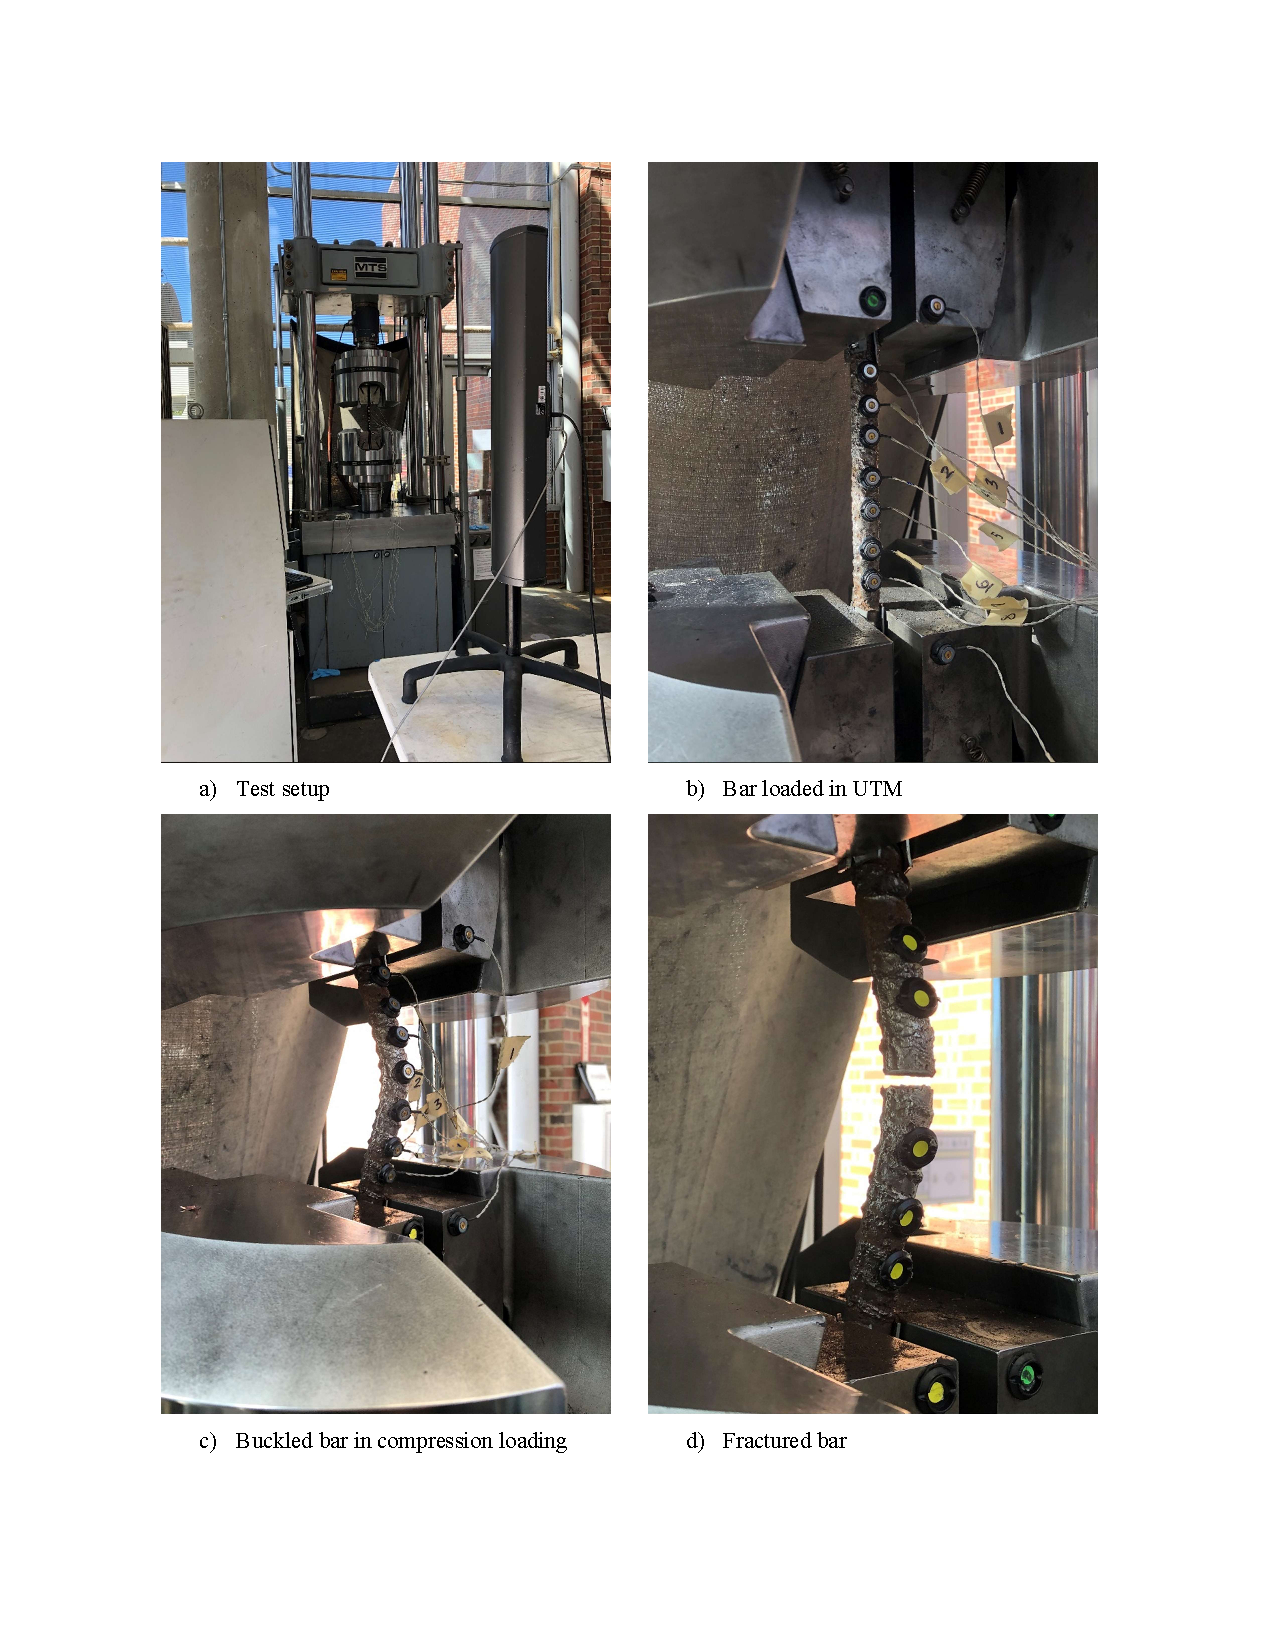
\includegraphics[width=0.7\textwidth]{VAC Thesis 2.0/Chapter-4/figs/BBT Procedure.pdf}
	\caption{General procedure of buckled bar tension (BBT) test}
	\label{fig:BBT_Test_Summary}
\end{figure}

The data obtained from the BBT test is then procesed and two parameters are obtained: 1) the cirtical bending strain, based on the curvature, 2) the maximum uniform axial deformation is obtained from the stress strain curve. This two values are obtained as shown in \fref{fig:bendingstrain}. In the case of brittle failure if the bar does not elongate compared to its original length the uniform axial elongation is assigned a value of zero.

\begin{figure}[htbp]
	\centering
	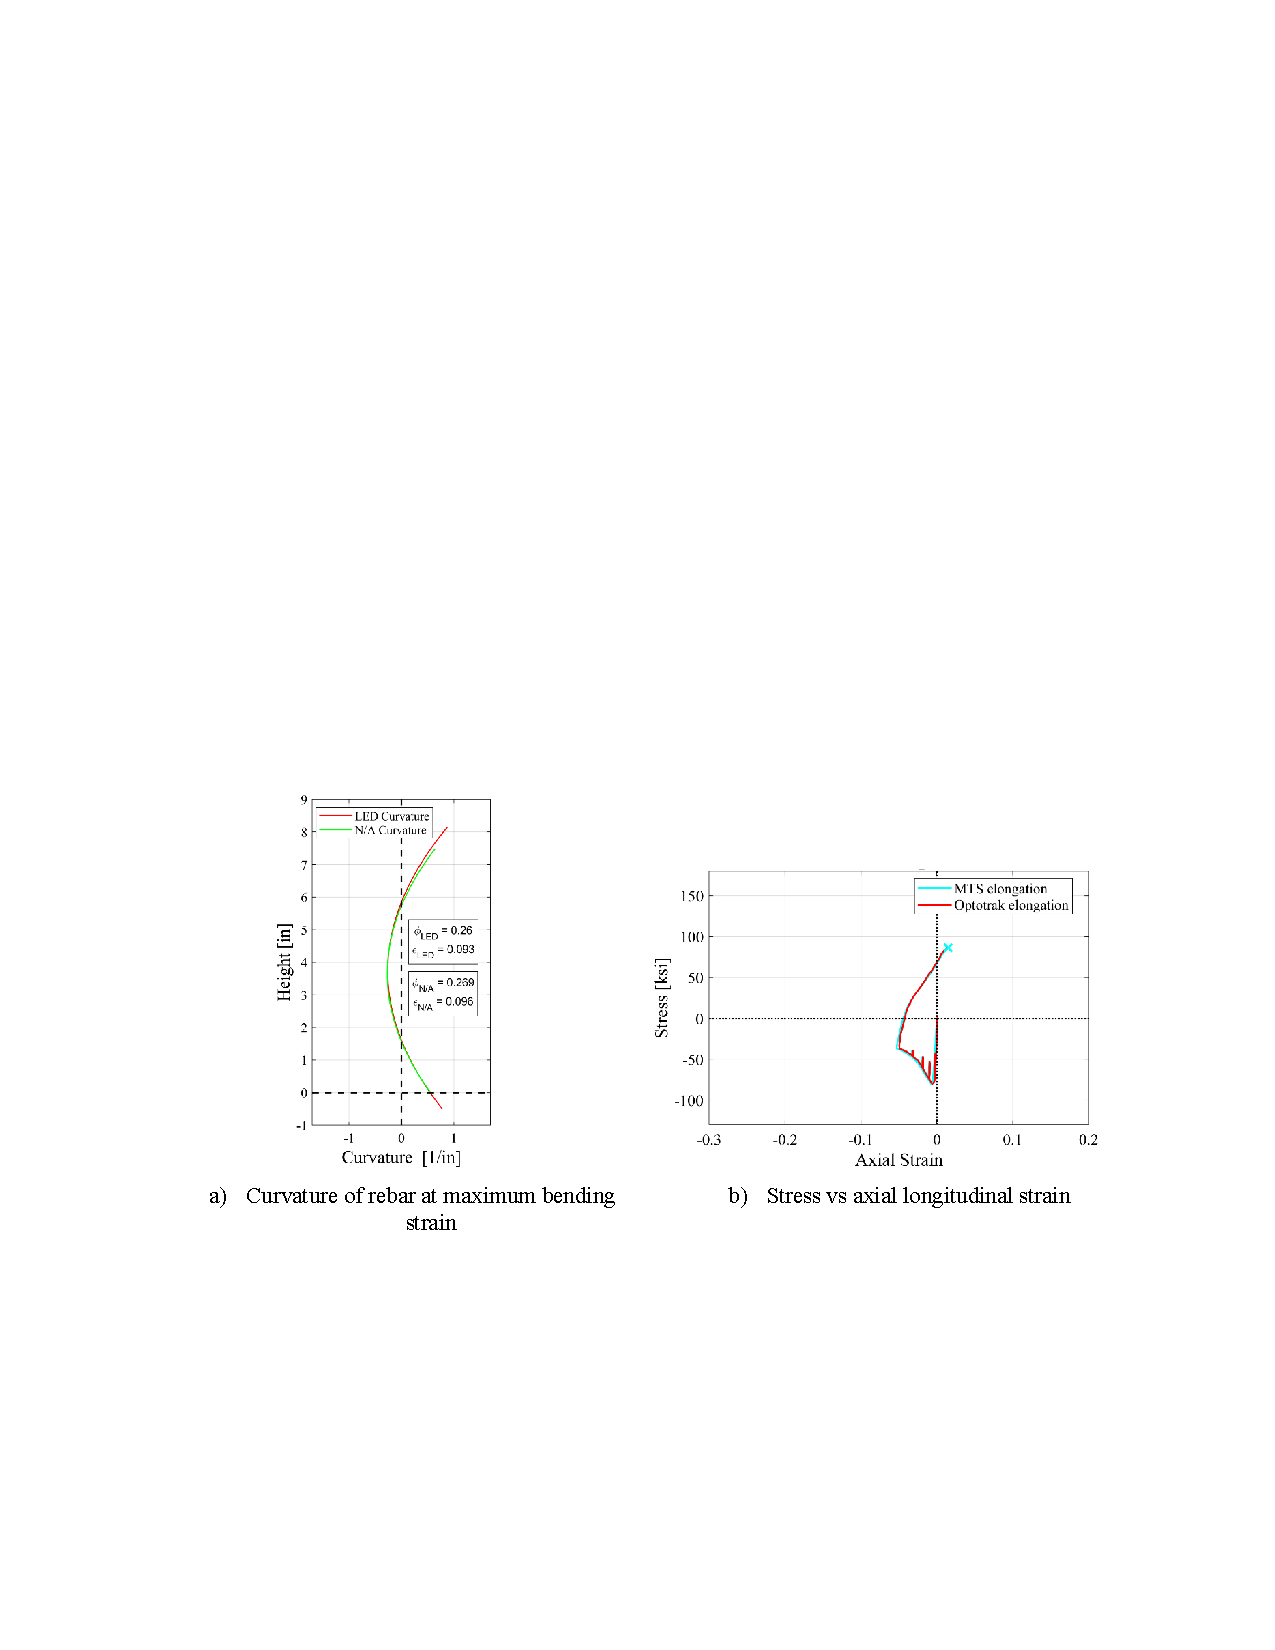
\includegraphics[width=1\textwidth]{VAC Thesis 2.0/Chapter-4/figs/BBT_curvature.pdf}
	\caption{Obtaining critical bending strain}
	\label{fig:bendingstrain}
\end{figure}

\subsection{Effect of corrosion in Critical Bending Strain}

The buckled bar tension test was applied to rebars with varying levels of corrosion ranging from 0\% - 20\%. For each corrosion level a total of 6 BBT tests was performed, plotting the bending strain vs the uniform axial elongation, the critical bending strain is calculated as the point where the uniform axial elongation drops to zero. \fref{fig:BBT_strains} summarizes the critical maximum bending strain at different corrosion levels including the benchmark value of pristine bars obtained by Barcley et al \cite{Barcley2018}. In \fref{fig:eb_vs_CL} it is noticible that as corrosion level increases the maximum bending strain reduces.

\begin{figure}[htbp]
	\centering
	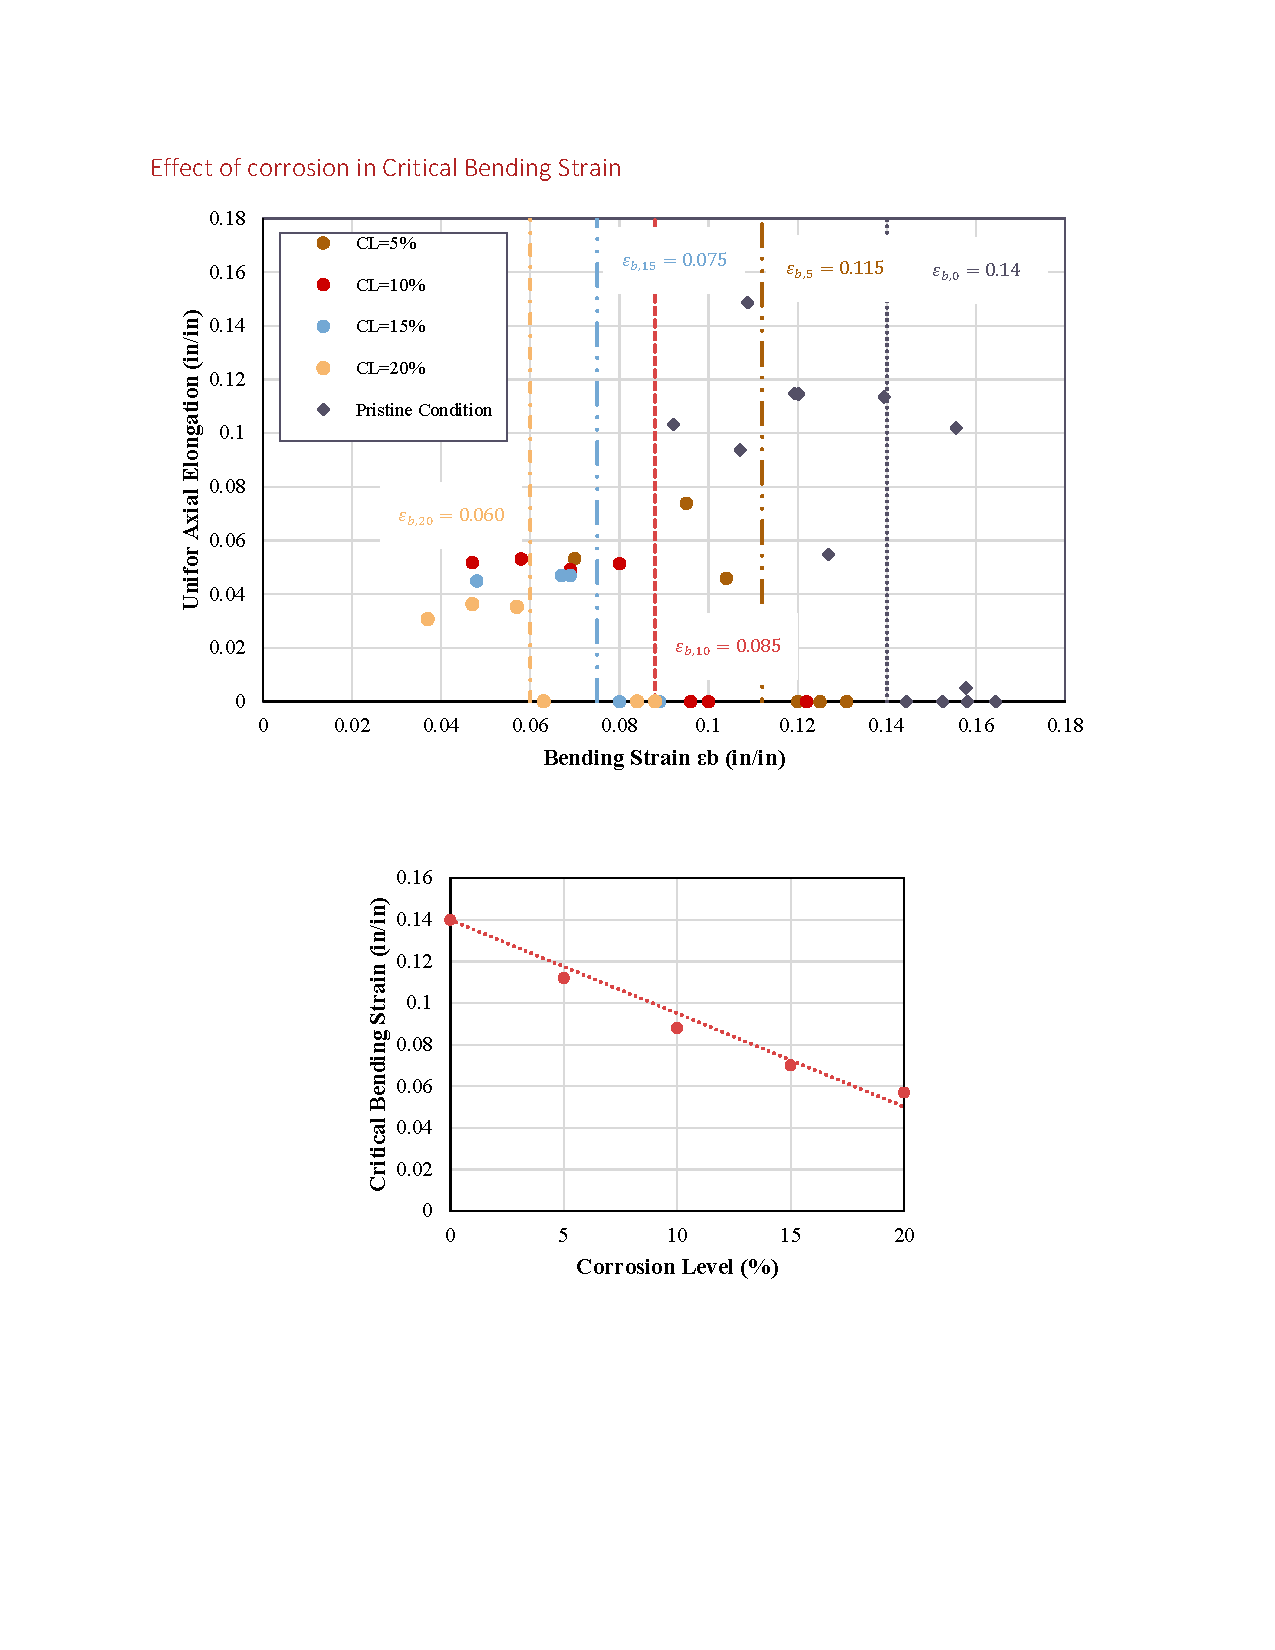
\includegraphics[width=0.7\textwidth]{VAC Thesis 2.0/Chapter-4/figs/BBT_results_.pdf}
	\caption{Bending strain at different corrosion levels}
	\label{fig:BBT_strains}
\end{figure}

\fref{fig:eb_vs_CL} shows the relationship between the critical bending strain and the corrosion level of the rebars. There is a linear relationship between both variables similar to the one observed in the tension tests.The relationship between corrosion level and cirtical bending strain ($\varepsilon_{b}$) using linear regression can be expressed as shown below in \ref{eq.Calderon_eb_vs_CL}.

\begin{equation}
    \varepsilon_{b}(CL) = \varepsilon_{o}-0.0045CL
    \label{eq.Calderon_eb_vs_CL}
\end{equation}

It is interesting to notice the sharp drop in critical bending strain capacity as corrosion increases. For CL=5\% There is a drop of about 20\%, for CL=10\% the change is 60\% of the pristine condition and for CL=20\% that difference is more than 140\% decrease in the critical bending strain. This results indicate that there is a reduction in the ultimate capacity of rebars as they corrode. Based on this results and previous tests performed in corroded RC beams reported by Du et al \cite{Du2005}, on RC columns as shown by Ma et al \cite{Ma2012} and Meda et al \cite{Meda2014}, a limiting value for level of corrosion is CL=10\%.

\begin{figure}[htbp]
	\centering
	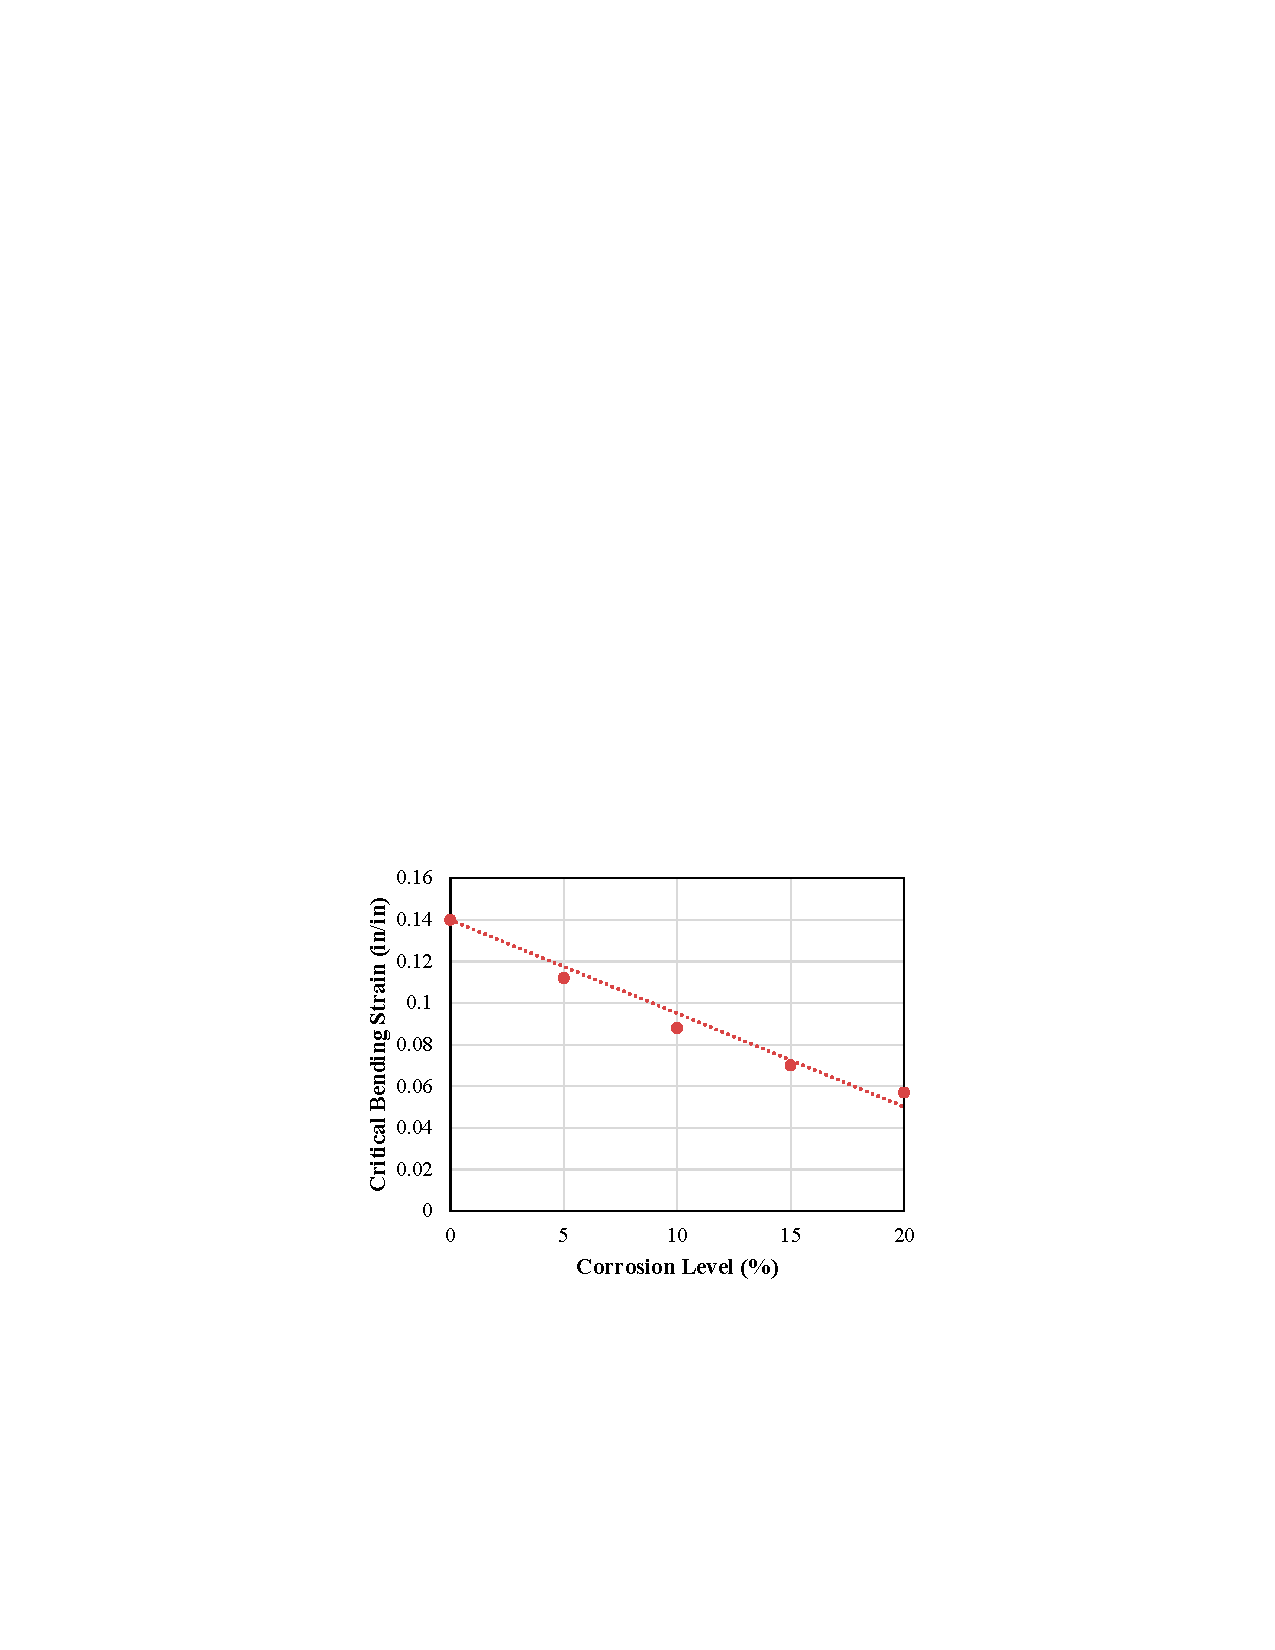
\includegraphics[width=0.7\textwidth]{VAC Thesis 2.0/Chapter-4/figs/BBT_results_summary.pdf}
	\caption{Maximum bending strain as a function of corrosion level}
	\label{fig:eb_vs_CL}
\end{figure}

\subsection{Effect of corrosion at the micro-structural level}

To study if there was any change in the microstructural behavior of the rebars as they corroded and explore if the chlorides induced fracture in the rebars at the point of fracture, the rebar's fracture surfaces were observed under a variable pressure scanning electron microscope (VPSEM). Fracture surfaces from ductile and brittle failures were obtained at ductility levels of 5\%-20\%.

\textbf{Fractography of BBT test specimens fracture surfaces}

 As previously observed in figure X, at the macro level brittle fractures typically consist of flat fracture surface, and in ductile fractures, there is necking and rougher edges along the fracture surface. The observations at the macro level translate into similar observations at the microstructural level. To analyze the images obtained from the Scanning Electron Microscope (SEM), it is important to understand how brittle and ductile fractures in metals look like in the SEM. \fref{fig:fractography101} summarizes the typical features for brittle fractures and ductile fractures. Brittle fractures, present features that tend to promote flat surfaces, that two main types are granular and cleavage fractures. Ductile fractures on the other hand have dimple features, which due to the extension of the fracture surface at the point where atomic bonds are broken.
 
\begin{figure}[htbp]
	\centering
	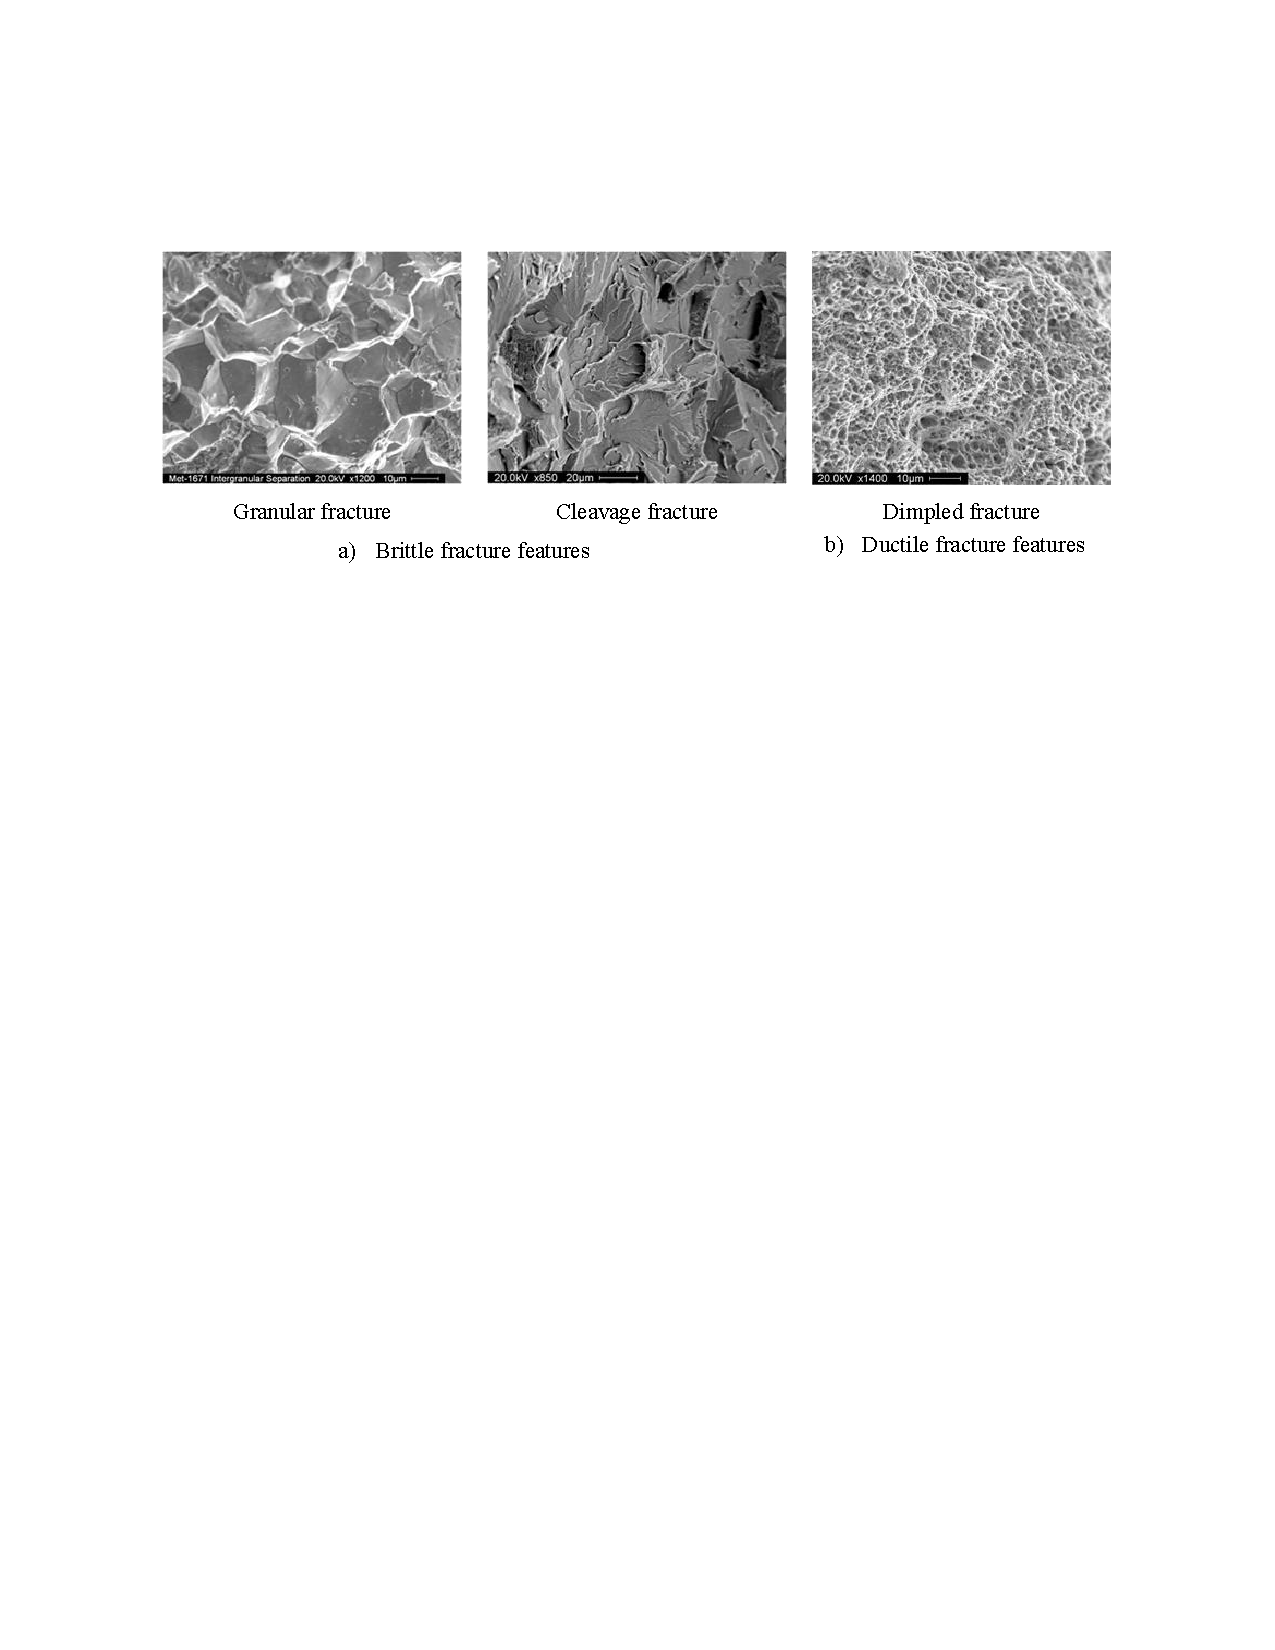
\includegraphics[width=0.825\textwidth]{VAC Thesis 2.0/Chapter-4/figs/FractographyBasics_101.pdf}
	\caption{Basic features analysis of fracture surfaces in metals}
	\label{fig:fractography101}
\end{figure}

\fref{fig:FractureSurfaces} summarizes the observations performed on the fracture surfaces.  While VPSEM images were obtained for each corrosion level no substantial differences for brittle and ductile samples was observed as the corrosion level increased. Therefore, the observations performed on the CL=10\% samples are shown here as representative of all the observations. The methodology of the observations was in such a way that differences between different sectors of the fracture provided comparison points. \fref{fig:FractureSurfaces} shows three main sectors 1) point of initiation of fracture, 2) midpoint and 3) the extreme fiber opposite to the initiation of fracture. In all cases the point of initiation of fracture occurred where the extreme fiber was subjected to tension while being compressed. 

Comparing the images obtained for the brittle and ductile response in \fref{fig:FractureSurfaces} we can make the following observations. 1) At the point of initiation of fracture for the brittle and ductile surfaces there is no difference in the behavior of the fracture surfaces observed, indicating that the point of initiation of fracture is always brittle in nature, this can be seen in the presence of flat surfaces. 2) At the midpoint we can start to observe some differences for the brittle sample, flat surfaces are still observed but for the ductile sample, a mixture of flat surfaces and dimples typical of ductile surfaces are observed, this mixture of responses is similar to SEM observations of fracture surfaces of fatigue fractures. And 3) At the extreme fiber point the difference between ductile and brittle is more prominent since the ductile response has a predominant presence of dimples and the  brittle response still shows flat surfaces. This results tell us the different mechanisms that occur between the brittle and ductile response and correlate well with the observed behavior of the BBT tests.

\begin{figure}[htbp]
	\centering
	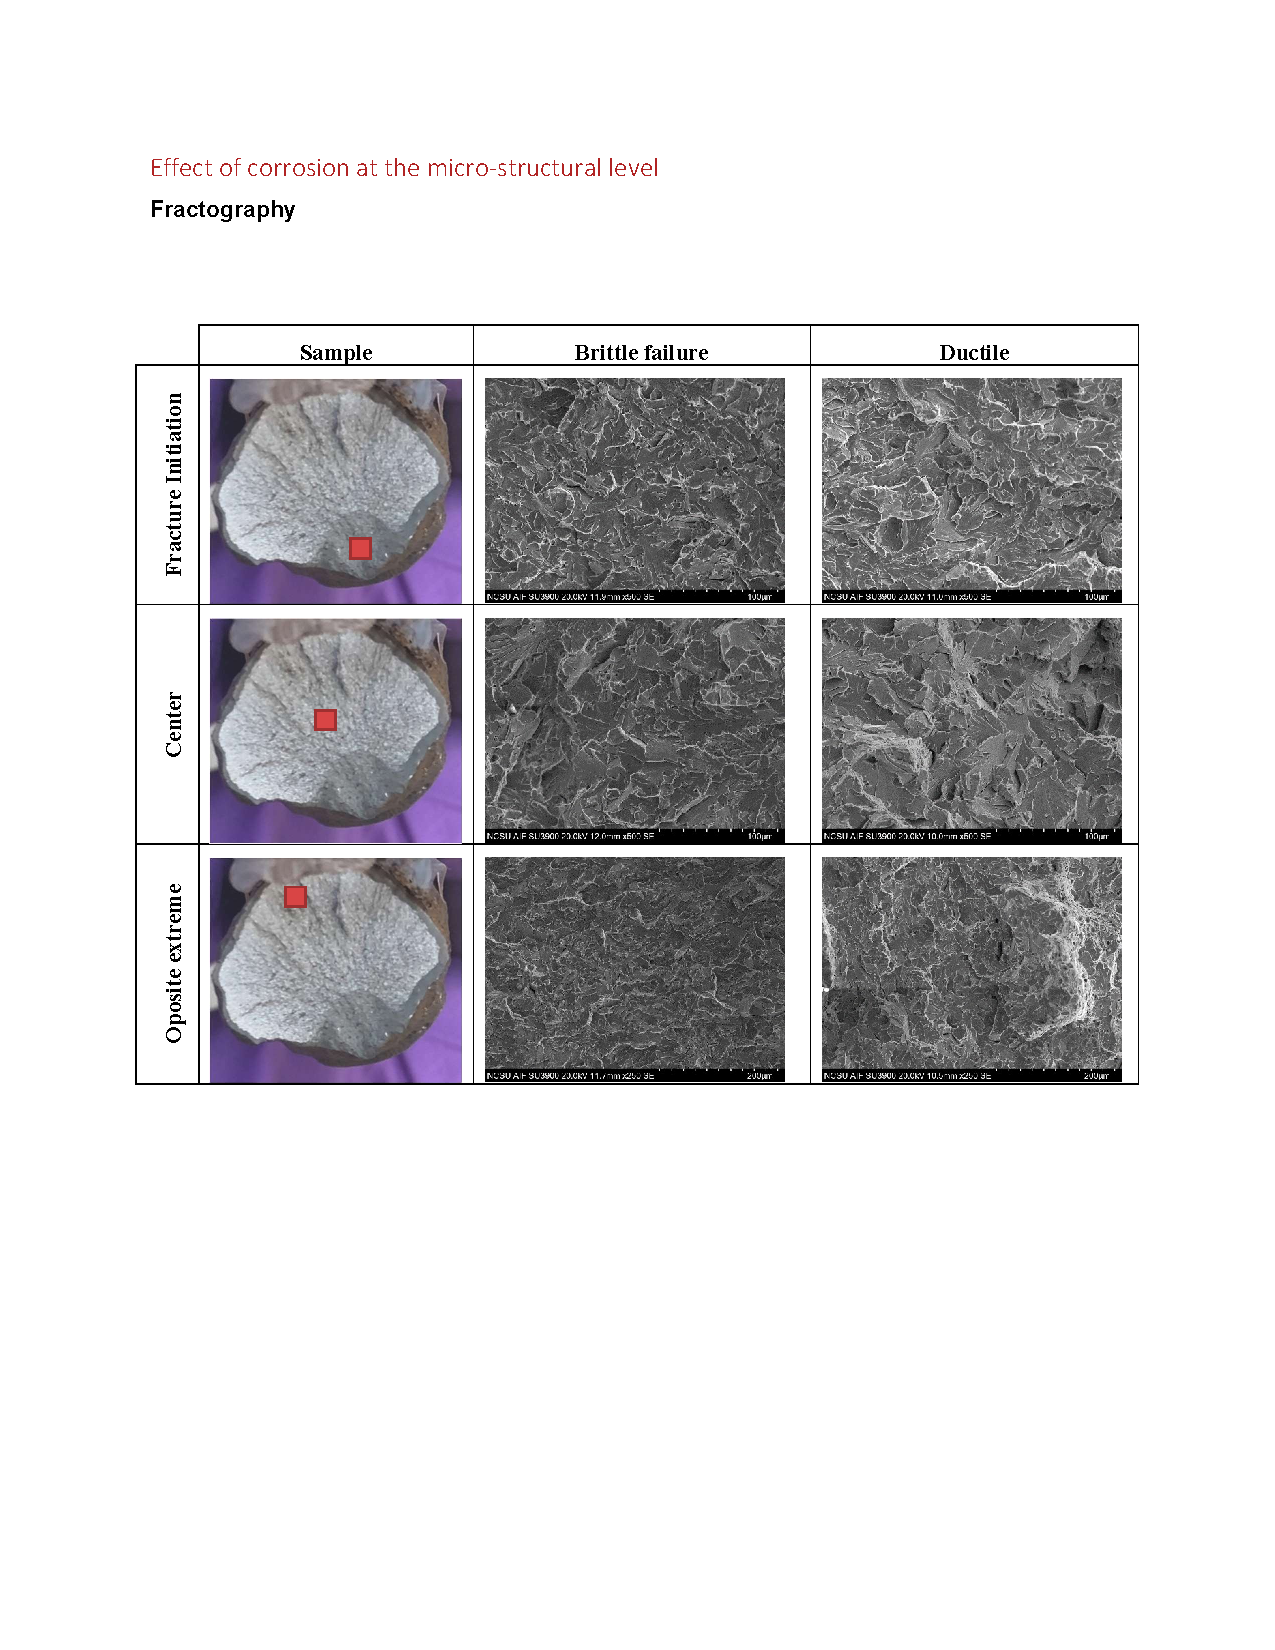
\includegraphics[width=1\textwidth]{VAC Thesis 2.0/Chapter-4/figs/BBT_fractography.pdf}
	\caption{SEM observations for brittle and ductile failure at different positions of the fracture surface}
	\label{fig:FractureSurfaces}
\end{figure}

An important feature from the images obtained in the VPSEM observations was river like features observed throught all the points of observations, as shown in \fref{fig:RiverFeatures}. This type of features is typical of cyclic of fatigue  tests, which is coherent with the BBT tests since the bar is loaded in compression and then loaded in tension. %Expand on this and include pictures from Hull Book to explain this type of feature and the information found on the ASME website

\begin{figure}[htbp]
	\centering
	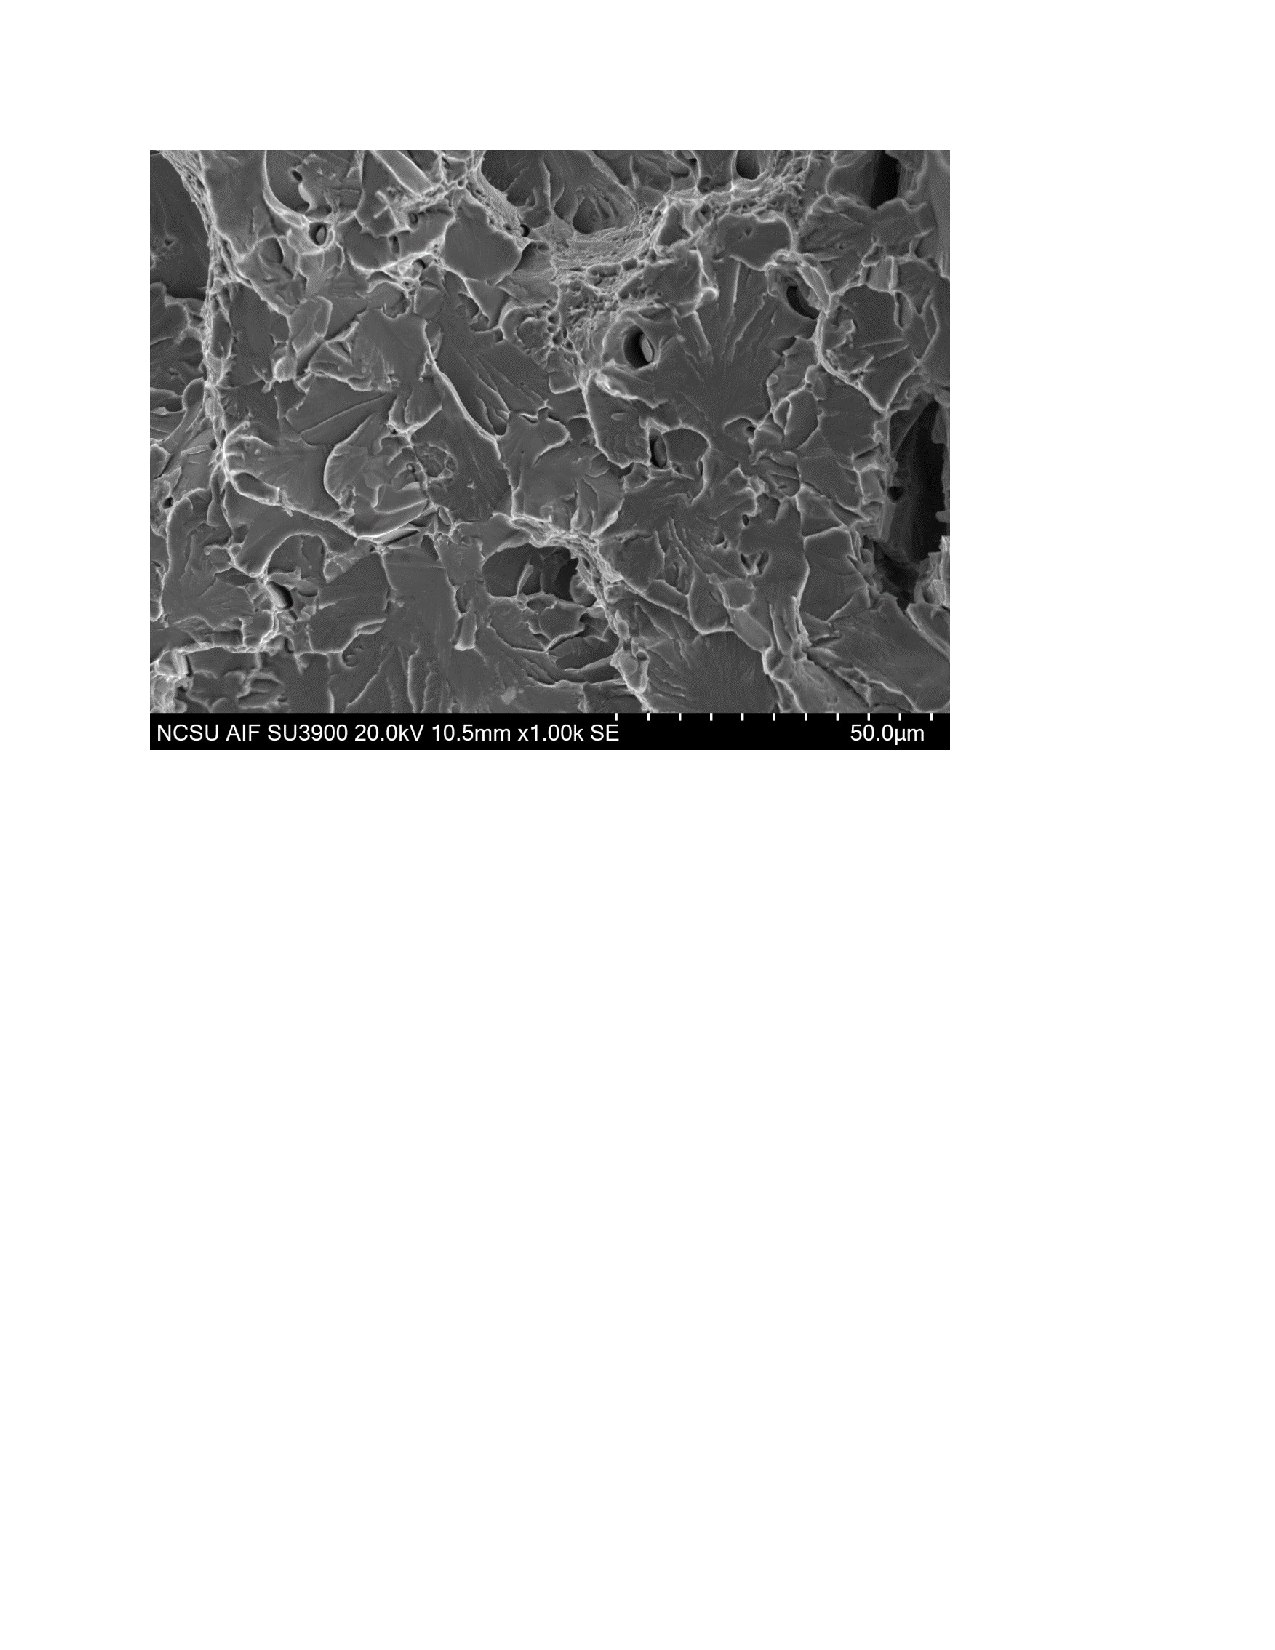
\includegraphics[width=0.7\textwidth]{VAC Thesis 2.0/Chapter-4/figs/BBT_RiverFeatures.pdf}
	\caption{SEM cyclic loading features in fracture surface at 500x magnification}
	\label{fig:RiverFeatures}
\end{figure}

\newpage
\textbf{Spectrum analysis}

In order to rule out the preclusion to failure due to inclusion of chlorides in the fracture surface a Back Scatter Electron (BSE) SEM images were evaluated through the use of spectrum analysis of the X-ray energy of the fracture surface. \fref{fig:SpectrumAnalysis} shows the spectrum analysis of a brittle and ductile sample. The results obtained show elements that are expected on alloyed steel such as iron (Fe), carbon (C), chromium (Cr), Manganese (Mn), and vanadium (V), among others. But no presence of chlorides (NaCl) of oxides(O) was detected. Thus ruling out the onset of fracture due to the presence of these compounds.

\begin{figure}[htbp]
	\centering
	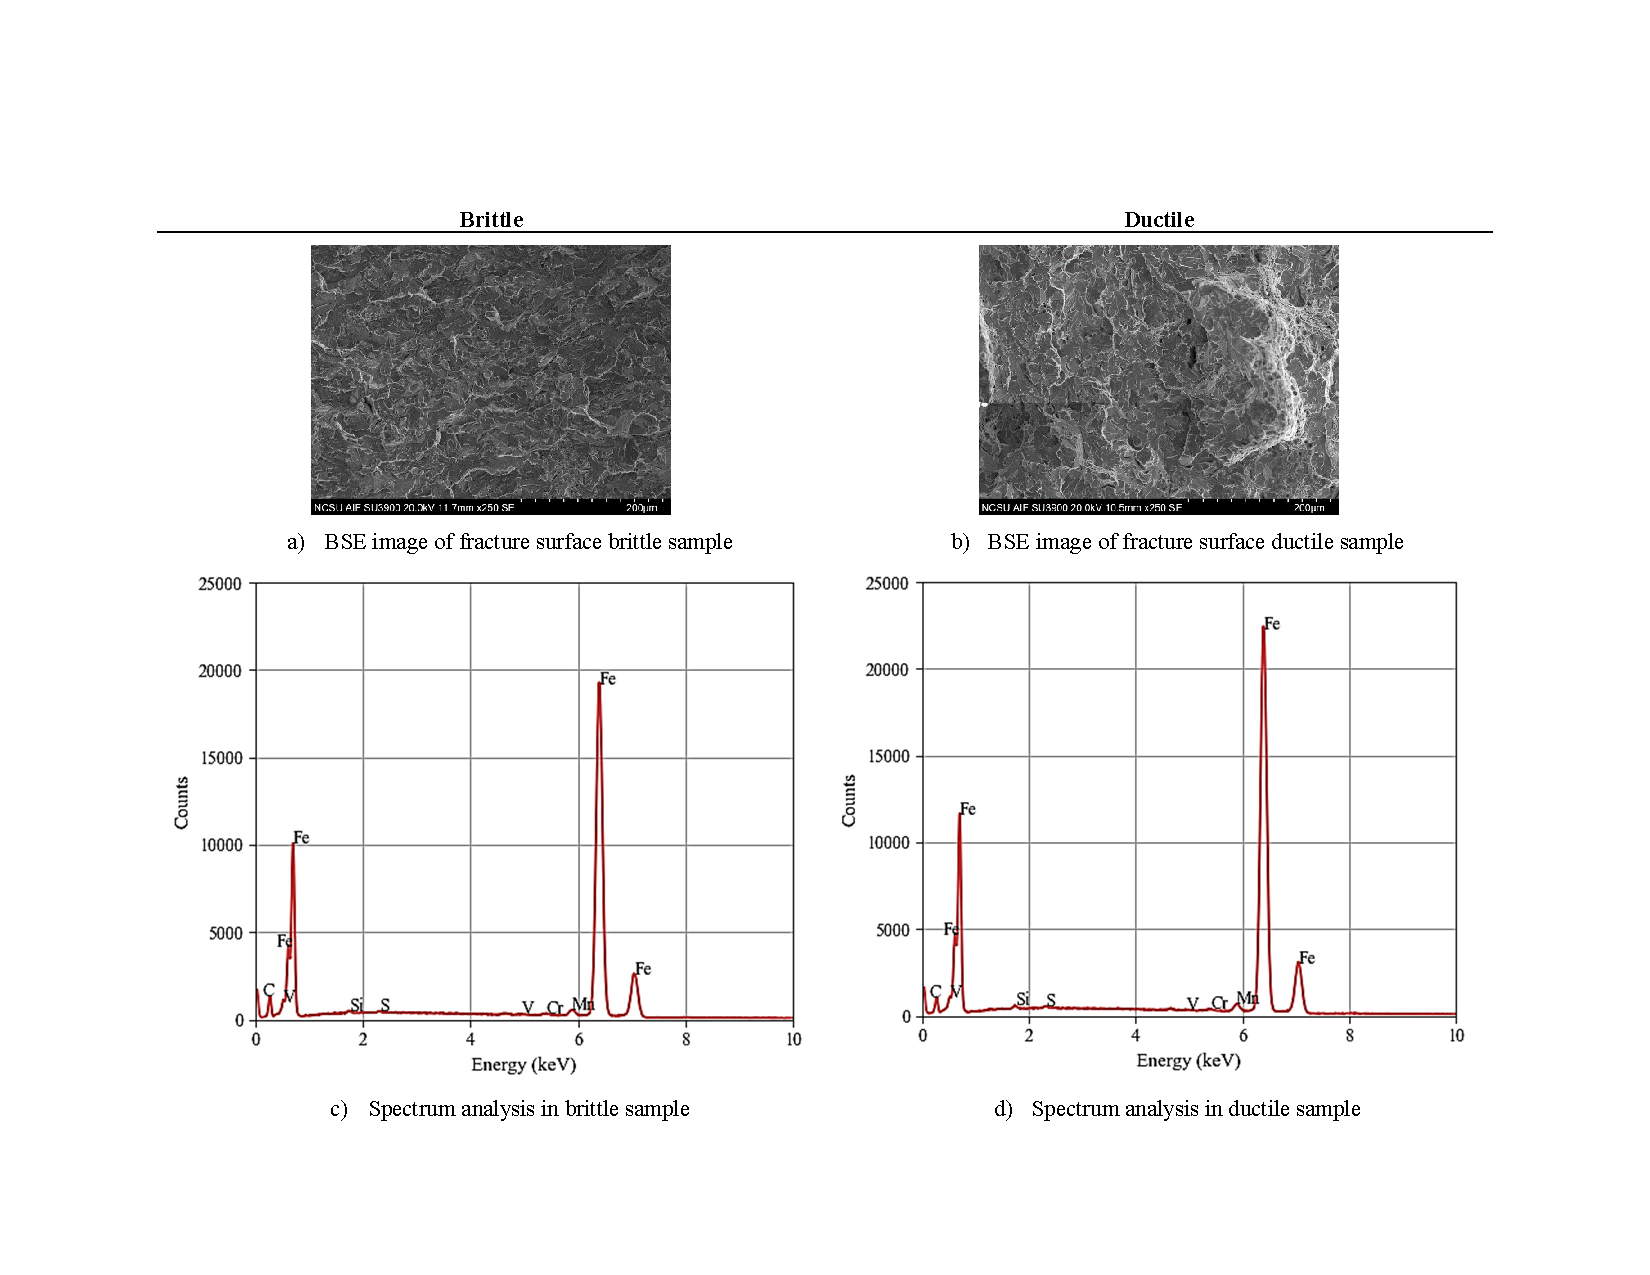
\includegraphics[width=0.9\textwidth]{VAC Thesis 2.0/Chapter-4/figs/BBT_SpectrumAnalysis.pdf}
	\caption{Spectrum analysis of Back Scatter Electrons of fracture surface for brittle and ductile failures}
	\label{fig:SpectrumAnalysis}
\end{figure}

\subsection{Effect of geometry imperfections}